\documentclass[12pt, a4paper]{article}
\usepackage[czech]{babel}
\usepackage{amsmath, amssymb}
\usepackage{tikz}
\usepackage{pgfplots}
\usepackage{float}
\usepackage{hyperref}
\usepackage{subcaption}
\usepackage{graphicx}
\usepackage{xcolor}
\usepackage{gensymb}
\graphicspath{ {./ryska} }
\usetikzlibrary{patterns}
\floatstyle{boxed} 
\restylefloat{figure}
\newcommand{\imply}{\Rightarrow}
\newcommand{\equiva}{\Leftrightarrow}

\title{Matematika pro sigmy}
\author{Fudži Mi Nagule}
\date{Únor 2025}

\begin{document}
\maketitle
\pagebreak
\begin{abstract}
Vypracované otázky z matematiky, tipy a triky a tak
\end{abstract}
\pagebreak

\tableofcontents

\pagebreak
\section{Výroková logika a množiny}

\subsection*{Množiny}
Množinou rozumíme souhrn nějakých objektů (prvků). Zápis $x \in M$ znamená že prvek \textit{x} náleží množině \textit{M}. Množinu můžeme určit výčtem prvků, charakteristickou vlastností nebo 
množinovými operacemi. Rovnost množin znamená, že každý prvek množiny \textit{M} je prvkem množiny \textit{N} a současně každý prvek množiny \textit{N} je prvkem množiny \textit{M}.

\subsubsection*{Podmnožina}
Množinu \textit{M} nazýváme podmnožinou množiny \textit{N}, právě když je každý prvek množiny \textit{M} prvkem množiny \textit{N}. Zápis symbolem $\subseteq$ nebo $\subset$; $M\subset N$ značí, že \textit{M} je vlastní podmnožinou množiny \textit{N}, tedy $M \neq N$; $M \subseteq N$ značí nevlastní podmnožinu, tedy $M \subset N$ nebo $M = N$.

\subsubsection*{Charakteristická vlastnost}
Zápis $A=\{x \in M; vlastnost\}$, kde každý prvek z množiny \textit{M}, mající danou vlastnost, patří do množiny \textit{A}.

\subsection*{Množinové operace}
\textbf{Sjednocení} $A \cup B$, je množina všech prvků, patřících alespoň do jedné z množin \textit{A}, \textit{B}.\\
\textbf{Průnik} $A \cap B$, je množina všech prvků, patřících zároveň do obou množin \textit{A}, \textit{B}.\\
\textbf{Rozdíl} $A \setminus B$, je množina všech prvků, patřících do množiny \textit{A} a \textbf{nepatřících} do množiny \textit{B}.\\
! Sjednocení i průnik jsou komutativní a asociativní operace.\\
\textbf{Doplněk} $A'_M $ množiny A v množině M je množina všech prvků množiny M, které nepatří do množiny A $\Rightarrow A'_M = M \setminus A$.

\subsection*{Intervaly}
Nechť \textit{a}, \textit{b} jsou dvě reálná čísla, že $a<b$, pak\\
$(a,b) = \{x \in \mathbb{R}; a < x < b\}$ je otevřený interval\\
$(a,b\rangle = \{x \in \mathbb{R}; a < x \leq b\}$ je polootevřený interval\\
$\langle a,b) = \{x \in \mathbb{R}; a \leq x < b\}$ je polouzavřený interval\\
$\langle a,b \rangle = \{x \in \mathbb{R}; a \leq x \leq b\}$ je uzavřený interval\\

\subsection*{Výroky}
Výrokem rozumíme sdělení, o kterém má smysl uvažovat jeho pravdivost. Každý výrok má \textbf{pravdivostní hodnotu}, 0 (nepravda) nebo 1 (pravda).\\
\textbf{Hypotéza} je výrok jehož pravdivostní hodnotu neznáme. \\
\textbf{Výroková formule} je tvrzení s proměnou, po dosazení se stane výrokem.

\subsubsection*{Negace výroku}
\textbf{Negace výroku}, \textit{"Není pravda, že A"}, zapisujeme $\neg A $, vždy opačná pravdivostní hodnota.

\subsubsection*{Logické operátory}
Pomocí těchto operátorů tvoříme \textbf{složené výroky} nebo \textbf{formule}.\\
\textbf{Konjunkce}, "A a současně (et) B", zapisujeme $A \land B$
\begin{center}
\begin{tabular}{|c | c | c|} 
\hline
A & B & $A \land B$ \ \\
\hline
0 & 0 & 0 \\
\hline
0 & 1 & 0 \\
\hline
1 & 0 & 0 \\
\hline
1 & 1 & 1\\
\hline
\end{tabular}
\end{center}
\textbf{Disjunkce}, "A nebo (vel) B", zapisujeme $A \lor B$
\begin{center}
\begin{tabular}{|c | c | c|} 
\hline
A & B & $A \lor B$ \ \\
\hline
0 & 0 & 0 \\
\hline
0 & 1 & 1 \\
\hline
1 & 0 & 1 \\
\hline
1 & 1 & 1\\
\hline
\end{tabular}
\end{center}
\textbf{Ostrá disjunkce}, "Buď A, nebo B", zapisujeme $ A \veebar B $
\begin{center}
\begin{tabular}{|c | c | c|} 
\hline
A & B & $A \veebar B$ \ \\
\hline
0 & 0 & 0 \\
\hline
0 & 1 & 1 \\
\hline
1 & 0 & 1 \\
\hline
1 & 1 & 0\\
\hline
\end{tabular}
\end{center}
\textbf{Implikace}, "Z A plyne B", zapisujeme $A \Rightarrow B$
\begin{center}
\begin{tabular}{|c | c | c|} 
\hline
A & B & $A \Rightarrow B$ \ \\
\hline
0 & 0 & 1 \\
\hline
0 & 1 & 1 \\
\hline
1 & 0 & 0 \\
\hline
1 & 1 & 1\\
\hline
\end{tabular}
\end{center}
\textbf{Ekvivalence}, "A je ekvivalentní s B.", "A právě tehdy, když B.", zapisujeme $A \Leftrightarrow B$ 
\begin{center}
\begin{tabular}{|c | c | c|} 
\hline
A & B & $A \Leftrightarrow B$ \ \\
\hline
0 & 0 & 1 \\
\hline
0 & 1 & 0 \\
\hline
1 & 0 & 0 \\
\hline
1 & 1 & 1\\
\hline
\end{tabular}
\end{center}

\subsubsection*{Tautologie}
\textbf{Tautologie} je výrok/formule, který je vždy pravdivý.\\ 
\textbf{Kontradikce} je výrok/formule, který je vždy nepravdivý.\\
\textbf{Důležité tautologie}:
\begin{itemize}
\item $\neg(\neg A) \equiv A$ 
\item $\neg (A \Rightarrow B) \equiv A \land \neg B$ 
\item $ A \Rightarrow B \equiv \neg B \Rightarrow \neg A $
\item $ \neg (A \land B) \equiv \neg A \lor \neg B$
\item $ A \Rightarrow B \equiv \neg A \lor B $
\item $ \neg (A \Leftrightarrow B) \equiv A \veebar B $
\item $ \neg (A \lor B) \equiv \neg A \land \neg B $
\item $ A \Leftrightarrow B \equiv (A \Rightarrow B) \land (B \Rightarrow A) $
\item $ \neg (A \veebar B) \equiv A \Leftrightarrow B$
\end{itemize}
\pagebreak

\subsection*{Kvantifikace výrokových formulí}
Výroková formule $\varphi (x)$, obsahující proměnnou x, se stane výrokem po kvantifikaci \textit{x}.\\
\textbf{Obecný kvantifikátor} $\forall$, "pro každé, pro všechna, ..." \\
\textbf{Malý kvantifikátor} $\exists$, "existuje alespoň jedno, nějaké, ..." \\
Př.: Formuli $\varphi (x) \sim x > 0$ lze kvantifikovat:\\
$(\forall x \in \mathbb{N}) x > 0$ ... Všechna přirozená čísla jsou kladná.\\
$ (\exists x \in \mathbb{N}) x > 0$ ... Existuje alespoň jedno přirozené číslo větší než 0.\\

\subsubsection*{Negace kvantifikátorů}
Negace výroku $(\forall x) \varphi (x) $ je výrok $(\exists x) \neg \varphi (x)$.\\
Negace výroku $(\exists x) \varphi (x) $ je výrok $ (\forall x) \neg \varphi (x)$.\\

\subsection*{Věta, definice, důkaz, správné úsudky}
\textbf{Matematická věta} je důležité, netriviální a dostatečně obecné tvrzení neboli výrok. Věta obsahuje předpoklad a závěr.
\textbf{Axiom (postulát)} je tvrzení, které se předem předpokládá za platné. 
\textbf{Definice} slouží k zavedení nových pojmů; stanoví nový pojem a určí ho pomocí již stanovených.
\subsubsection*{Správný úsudek}
\textbf{Správný úsudek} je takový, kdy je z pravdivých premis vyvozen pravdivý závěr.\\
\textbf{Zákon vyloučení možnosti}:
\begin{gather*}
 p \lor q \\ \neg p \\ \hline q
\end{gather*}
\textbf{Zákon odloučení}:
\begin{gather*}
p \Rightarrow q \\ p \\ \hline q
\end{gather*}
\textbf{Zákon nepřímé úvahy}:
\begin{gather*}
p \Rightarrow q \\ \neg q \\ \hline \neg p
\end{gather*}
\textbf{Zákon kontrapozice}:
\begin{gather*}
p \Rightarrow q \\ \hline \neg q \Rightarrow \neg p
\end{gather*}
\pagebreak
%-----------------------------------------------------------------------------------------------------------------------------------------------------------------------------------------------------------%
\section{Mnohočleny, mocniny a odmocniny}

Zápis $ 1 + \sqrt{1,5625-(\frac{3}{4})^2} $ je \textbf{číselný výraz} s hodnotou 2.\\
Zápis $ x^2 + 2xy +1 $ je výraz s proměnnými \textit{x}, \textit{y}.\\
\textbf{Definiční obor výrazu} je množina všech přípustných hodnot proměnné, pro které má výraz smysl.\\
Výraz $V = x^2 +1 $ má definiční obor $\mathbb{R}$\\
Výraz $V = \frac{1}{y}$ má smysl pro nenulové hodnoty \textit{y} \\
 $\Rightarrow D_V : y \in \mathbb{R} \setminus \{0\}$  nebo $ D_V = (-\infty,0) \cup (0,+\infty)$\\

\subsection*{Mnohočleny}
\textbf{Mnohočlen} (polynom) s jednou proměnnou je výraz $ a_nx^n + a_{n-1}x^{n-1} +...+ a_1x^1 + a_0 $, kde \textit{n} je stupeň mnohočlenu.\\
$a_1x + a_0$, resp. $ax+b$ je linearní dvojčlen.\\
$a_2x^2 + a_1x + a_0$, resp. $ax^2 + bx + c$ je kvadratický trojčlen.\\

\subsubsection*{Dělení mnohočlenu mnohočlenem}
$(4x^3 + 3x^2 - 2x -5):(x-1) = 4x^2 + 7x + 5$\\
$ 4x^3 - 4x^2$\\
\rule{2cm}{0.4pt}\\
$ 0x^3 + 7x^2 -2x$\\
$ 0x^3 + 7x^2 -7x$\\
\rule{3cm}{0.4pt}\\
$0x^3 + 0x^2 + 5x - 5$\\
$0x^3 + 0x^2 + 5x - 5$\\
\rule{4cm}{0.4pt}\\
$0x^3 + 0x^2 + 0x - 0$\\
pozn. zbytek stejně jako u číselného dělení\\

\subsubsection*{Umocňování}
\begin{itemize}
\item $(AB)^n = A^nB^n$
\item $(A+B)^2 = A^2 + 2AB + B^2$
\item $(A-B)^2 = A^2-2AB+B^2$
\item $(A+B)^3=A^3 + 3A^2B + 3AB^2 + B^3$
\item $(A-B)^3=A^3 - 3A^2B + 3AB^2 - B^3$
\item $A^2-B^2 =(A-B)(A+B)$
\item $A^3-B^3 = (A-B)(A^2+AB+B^2)$
\item $A^3+B^3 = (A+B)(A^2-AB+B^2)$
\item $(-A+B)^2 = (A-B)^2$
\item $(-A-B)^2 = (A+B)^2$
\item $(A+B)^n=\sum \binom{n}{k} a^{n-k}b^k $
\end{itemize}

\section{Lomené výrazy}
\subsection*{Rozšiřování a krácení lomených výrazů}
\textbf{Rozšířit lomený výraz} znamená vynásobit čitatele i jmenovatele stejným číslem.\\
\begin{center}
$\frac{x}{x+2}=\frac{x(x-2)}{(x+2)(x-2)}=\frac{x^2-2x}{x^2 - 4}$\\
\end{center}
\textbf{Krátit lomený výraz} znamená vydělit čitatele i jmenovatele stejným číslem.\\
\begin{center}
$\frac{a^2bc^3}{abc^2}=\frac{a^2bc^3:abc}{abc^2:abc}=\frac{ac^2}{c}=ac$\\
\end{center}

\subsection*{Sčítání a odčítání lomených výrazů}
Nejdříve rozložíme všechny jmenovatele na součin, určíme společný jmenovatel jako NSN všech jmenovatelů, každý LV rozšíříme na společný jmenovatel, sečteme a odečteme čitatele, rozložíme čitatele na součin a zkrátíme (je-li to možné) a určíme podmínky.\\
\[
\begin{aligned}
	V &= \frac{3+2x}{2-x}-\frac{2-3x}{2+x}+\frac{x(16-x)}{x^2-4}\\
	V &= \frac{3+2x}{2-x}-\frac{2-3x}{2+x}+\frac{x(16-x)}{(x+2)(x-2)}\\
	V &=  -\frac{(3+2x)(x+2)}{(x-2)(x+2)}-\frac{(2-3x)(x-2)}{(x+2)(x-2)}+\frac{x(16-x)}{(x+2)(x-2)}\\
	V &= \frac{-7x-6-2x^2-8x+4+3x^2+16x-x^2}{(x-2)(x+2)}\\
	V &= \frac{x-2}{(x-2)(x+2)}\\
	V &= \frac{1}{x+2}\\
\end{aligned}
\]

\subsection*{Vyjadřování neznámé ze vzorce}
Při vyjadřování neznámé ze vzorce využíváme:
\begin{itemize}
	\item záměna stran vzorce
	\item vynásobení/vydělení vzorce nenulovým číslem nebo výrazem
	\item přičtení/odečtení libovolného čísla nebo výrazu
	\item pokud jsou ve vzorci nezáporné veličiny, pak umocnění nebo odmocnění
\end{itemize} 

\subsection*{Výrazy s mocninami a odmocninami}
Pro každá reálná \textit{a}, \textit{b} a pro každá reálná \textit{r}, \textit{s} platí:
\begin{itemize}
	\item $a^r \cdot a^s = a^{r+s}$
	\item $ (a^r)^s = a^{r \cdot s} $
	\item $ \frac{a^r}{a^s} = a^{r-s} $
	\item $ (ab)^r = a^rb^r $
	\item $ (\frac{a}{b})^r = \frac{a^r}{b^r} $
	\item $ a^0 = 1, a \neq 0 $
	\item $ a^{-r} = \frac{1}{a^r} $
	\item $ \sqrt [s]{a^r} = a^{\frac{r}{s}}$
\end{itemize}
%-----------------------------------------------------------------------------------------------------------------------------------------------------------------------------------------------------------%
\section{Lineární rovnice a nerovnice}

\subsection*{Lineární rovnice}
\textbf{Lineární rovnice} má tvar $ax+b=0, a \neq 0$. Má jediný kořen $x=-\frac{b}{a}$.\\
Pokud užitím ekvivalentních úprav získáme tvar $0x+b=0$, pak má rovnice nekonečně mnoho řešení ($b=0$), nebo nemá řešení ($b \neq 0$).\\
\textbf{Definiční obor rovnice} je množina všech přípustných hodnot jejích kořenů; $x_1 \notin D_r \imply x_1 \notin K$.\\

\subsection*{Lineární nerovnice}
\textbf{Lineární nerovnice} má tvar: 
\begin{itemize}
\item $ax + b < 0$
\item $ax + b > 0$
\item $ax + b \leq 0$
\item $ax + b \geq 0$
\end{itemize}
Pokud lze nerovnici převést na tvar $ax + b \leq 0$:
\begin{center}
$b \leq 0 \imply K = \mathbb{R} \lor b > 0 \imply K = \{\}$
\end{center}
Pokud lze nerovnici převést na tvar $ax + b \geq 0$:
\begin{center}
$b \geq 0 \imply K = \mathbb{R} \lor b < 0 \imply K = \{\}$
\end{center}
Pokud lze nerovnici převést na tvar $ax + b < 0$:
\begin{center}
$b < 0 \imply K = \mathbb{R} \lor b \geq 0 \imply K = \{\}$
\end{center}
Pokud lze nerovnici převést na tvar $ax + b > 0$:
\begin{center}
$b > 0 \imply K = \mathbb{R} \lor b \leq 0 \imply K = \{\}$
\end{center}
\pagebreak

\subsection*{Grafické řešení lineární rovnice a nerovnice}
\textbf{Lineární funkce} je funkce s předpisem $y=ax+b$\\
Rovnici převedeme na tvar $ax+b=cx+d$ a budeme uvažovat $f(x)=ax+b$ a $g(x)=cx+d$, kořen leží v $f(x) \cap g(x)$.\\
\begin{figure}[H]
\centering
\begin{tikzpicture}
%% init-xy
\draw[help lines, color=gray!30, dashed] (-3.5,-3.5) grid (3.5,3.5);
\draw[->,ultra thick] (-3.5,0)--(3.5,0) node[right]{$x$};
\draw[->,ultra thick] (0,-3.5)--(0,3.5) node[above]{$y$};
%% init-xy
\draw [blue] (-1.5,3.5) -- (3.5,-1.5);
\draw [blue] (-1.25,-3.5) -- (2.25,3.5);
\filldraw [red] (1,1) circle (2pt);
\end{tikzpicture}
\caption{2x-1=2-x}
\end{figure}

\textbf{Lineární nerovnici} řešíme podobně jako rovnici: převedeme na tvar $ax+b=cx+d$ a budeme uvažovat $f(x)=ax+b$ a $g(x)=cx+d$, nerovnice mohou mít jeden z tvarů:\\
\begin{center}
\begin{tabular}{c  c  c  c} 
$-x-1>2x-\frac{5}{2}$ & $-x-1<2x-\frac{5}{2}$ & $-x-1 \geq 2x-\frac{5}{2}$ & $-x-1 \leq 2x-\frac{5}{2}$\\
$f(x)>g(x)$ & $f(x)<g(x)$ & $f(x) \geq g(x)$ & $f(x) \leq g(x)$\\
$K = (-\infty, \frac{1}{2})$ & $K = (\frac{1}{2}, \infty)$ & $K = (-\infty, \frac{1}{2} \rangle $ & $K = \langle \frac{1}{2}, \infty) $\\
 
ad 2 &
ad 3 &
ad 4 &
ad 5 \\
\end{tabular}
\end{center}

% ad 2
\begin{figure}[H]
\centering
\begin{tikzpicture}
% init-xy
\draw[help lines, color=gray!30, dashed] (-3.5,-3.5) grid (3.5,3.5);
\draw[->,ultra thick] (-3.5,0)--(3.5,0) node[right]{$x$};
\draw[->,ultra thick] (0,-3.5)--(0,3.5) node[above]{$y$};
% draw funcs
\draw [blue] (-3.5,2.5) -- (2.5,-3.5);
\draw [blue] (-0.5,-3.5) -- (3,3.5);
% draw roots
\draw [red] (-3.5,0) -- (0.5,0);
\draw [red] (0.5,0) circle (3pt);
\draw [gray, densely dotted] (0.5,-1.5) -- (0.5,0);
\end{tikzpicture}
\caption{$-x-1>2x-\frac{5}{2}$}
\end{figure}

% ad 3
\begin{figure}[H]
\centering
\begin{tikzpicture}
%% init-xy
\draw[help lines, color=gray!30, dashed] (-3.5,-3.5) grid (3.5,3.5);
\draw[->,ultra thick] (-3.5,0)--(3.5,0) node[right]{$x$};
\draw[->,ultra thick] (0,-3.5)--(0,3.5) node[above]{$y$};
%% init-xy
\draw [blue] (-3.5,2.5) -- (2.5,-3.5);
\draw [blue] (-0.5,-3.5) -- (3,3.5);
%draw roots
\draw [red]  (0.5,0) -- (3.5,0);
\draw [red] (0.5,0) circle (3pt);
\draw [gray, densely dotted] (0.5,-1.5) -- (0.5,0);
\end{tikzpicture}
\caption{ $-x-1<2x-\frac{5}{2}$ }
\end{figure}

% ad 4
\begin{figure}[H]
\centering
\begin{tikzpicture}
%% init-xy
\draw[help lines, color=gray!30, dashed] (-3.5,-3.5) grid (3.5,3.5);
\draw[->,ultra thick] (-3.5,0)--(3.5,0) node[right]{$x$};
\draw[->,ultra thick] (0,-3.5)--(0,3.5) node[above]{$y$};
%% init-xy
\draw [blue] (-3.5,2.5) -- (2.5,-3.5);
\draw [blue] (-0.5,-3.5) -- (3,3.5);
%draw roots
\draw [red] (-3.5,0) -- (0.5,0);
\filldraw [red] (0.5,0) circle (3pt);
\draw [gray, densely dotted] (0.5,-1.5) -- (0.5,0);
\end{tikzpicture}
\caption{$-x-1 \geq 2x-\frac{5}{2}$}
\end{figure}

% ad 5
\begin{figure}[H]
\centering
\begin{tikzpicture}
%% init-xy
\draw[help lines, color=gray!30, dashed] (-3.5,-3.5) grid (3.5,3.5);
\draw[->,ultra thick] (-3.5,0)--(3.5,0) node[right]{$x$};
\draw[->,ultra thick] (0,-3.5)--(0,3.5) node[above]{$y$};
%% init-xy
\draw [blue] (-3.5,2.5) -- (2.5,-3.5);
\draw [blue] (-0.5,-3.5) -- (3,3.5);
%draw roots
\draw [red]  (0.5,0) -- (3.5,0);
\filldraw [red] (0.5,0) circle (3pt);
\draw [gray, densely dotted] (0.5,-1.5) -- (0.5,0);
\end{tikzpicture}
\caption{$-x-1 \leq 2x-\frac{5}{2}$}
\end{figure}

\pagebreak

\subsection*{Rovnice a nerovnice v součinovém tvaru}
Při řešení využíváme $ab = 0 \equiva a = 0 \lor b = 0$.\\
Př.:\\
\[\begin{aligned}
x(x+2) = 0\\
x = 0 \lor x = -2\\
K = \{-2;0\}
\end{aligned}\]

Lze též použít \textbf{metodu nulových bodů}\\
Př.:\\
\[\begin{aligned}
4x^2 - 6x < 2x\\
4x^2 - 8x < 0\\
4x(x-2)<0\\
NB = \{0,2\}
\end{aligned}\]

\begin{center}
\begin{tabular}{| c | c | c | c |}
\hline
 & $(-\infty;0)$ & $(0;2)$ & $(2;+\infty)$\\
\hline
$4x$ & - & + & +\\
\hline
$x-2$ & - & - & +\\
\hline
$*$ & + & - & +\\
\hline
\end{tabular}
\end{center}

\[\begin{aligned}
K = (0;2)
\end{aligned}\]

\subsection*{Rovnice s neznámou ve jmenovateli}
Má-li rovnice neznámou ve jmenovateli, je nutné vždy stanovit její definiční obor.

\subsection*{Rovnice v podílovém tvaru}
Rovnice v podílovém tvaru má na jedné straně jediný zlomek s neznámou ve jmenovateli a na druhé straně nulu. Po stanovení definičního oboru řešíme rovnici tak,
že položíme čitatele rovno nule a řešíme jako lineární rovnici nebo převedením na součinový tvar.

\pagebreak

\subsection*{Nerovnice v podílovém tvaru}
\textbf{Nerovnici v podílovém tvaru nesmíme vynásobit společným jmenovatelem, který obsahuje neznámou!}\\
Nerovnici v podílovém tvaru převedeme na podílový tvar a řešíme metodou nulových bodů.\\
Př.:\\

\[
\begin{aligned}
\frac{2x-1}{x+1} \geq 1\\
x \neq -1\\
\frac{2x-1}{x+1} -1 \geq 0\\
\frac{2x-1-(x+1)}{x+1} \geq 0\\
\frac{x-2}{x+1} \geq 0\\
NB = \{-1,2\}
\end{aligned}\]

\begin{center}
\begin{tabular}{| c | c | c | c |}
\hline
 & $(-\infty;-1)$ & $(-1;2 \rangle $ & $ \langle 2;+\infty)$\\
\hline
$x-2$ & - & - & +\\
\hline
$x+1$ & - & + & +\\
\hline
$*$ & + & - & +\\
\hline
\end{tabular}
\end{center}

\[\begin{aligned}
K = (-\infty;-1) \cup \langle 2; +\infty)
\end{aligned}\]

\subsection*{Rovnice s absolutní hodnotou}
\textbf{Absolutní hodnota} z reálného čísla je definována jako\\
\[
   |a| =
    \begin{cases}
        a; & a \geq 0 \\
        -a; & a < 0
    \end{cases}
\]

Také platí :\\
\begin{itemize}

\item $|a|=|-a|$
\item $|a| \geq 0$
\item $|ab|=|a| \cdot |b|$
\item $|\frac{a}{b}| = \frac{|a|}{|b|}$
\end{itemize}

Nejprve určíme argumenty všech absolutních hodnot, ze kterých pak získáme nulové body a intervaly (u intervalu vždy ostrá závorka, kromě NB z jmenovatele). Poté vytvoříme
tabulku jako v tabulkové metodě. Řešíme s upravenými tvary dle definice. \textbf{Ukaždého kořenu musíme ověřit zda leží v intervalu!}\\
Př.:\\

\begin{center}
$|x-3| + 2x = 9$\\
\begin{tabular}{| c | c | c |}
\hline
$x \in $ & $(-\infty; 3 \rangle$ & $\langle 3; +\infty)$\\
\hline
$x-3$ & $-$ & $+$\\
\hline
$|x-3|$ & $(x-3)$ & $x-3$\\
\hline
\end{tabular}
\end{center}

\[
    \begin{array}{ll}
        \text{a)} & \hfill \text{b)}\\
         x \in (-\infty; 3 \rangle & \hfill x \in \langle 3; +\infty)\\
        -(x-3) + 2x = 9 & \hfill x - 3 + 2x = 9\\
        -x+ 3 + 2x = 9 & \hfill 3x - 3 = 9\\
        x = 6 & \hfill x = 4\\
        6 \notin (-\infty; 3 \rangle & \hfill 4 \in \langle 3; +\infty)\\
        K_1 = \{\} & \hfill K_2 = \{4\}\\
    \end{array}
\]\\
Rovnice má tedy jediný kořen $x=4$, tedy $K=\{4\}$.\\

Rovnici ve tvaru $|ax+b|=c$  lze řešit i \textbf{rychlejší metodou} bez stanovení intervalů, neboť platí $ax+b=c \lor ax+b=-c$.\\
I rovnici ve tvaru $|ax+b|=|cx+d|$ lze řešit touto rychlou metodou: $ax+b = cx+d \lor ax+b=-(cx+d)$.\\

\subsection*{Nerovnice s absolutní hodnotou}
Řešíme obdobně jako rovnici s absolutní hodnotou. Z argumentů určíme NB a řešíme nerovnice nahrezené dle definice. Množina řešení je sjednocení množin každého z případů.\\

\begin{center}
$|x+3|+3x<11$\\
\begin{tabular}{| c | c | c |}
\hline
$ x \in $ & $ (-\infty; 1 \rangle $ & $ \langle 1; + \infty) $\\
\hline
$x-1$ & $-$ & $+$\\
\hline
$|x-1|$ & $-(x-1)$ & $x-1$\\
\hline
\end{tabular}
\end{center}

\[
	\begin{array}{ll}
	\text{a)} & \text{b)}\\
	x \in (-\infty, 1 \rangle & \hfill x \in [1;+\infty)\\
	-(x-1) + 3x < 11 & \hfill x - 1 + 3x < 11\\
          -x + 1 + 3x < 11 & \hfill 4x < 12\\
          x < 5 & \hfill x < 3\\
	x \in (-\infty;5) & \hfill x \in (-\infty;3)\\
           K_1 = (-\infty; 1 \rangle \cap (-\infty;5) & \hfill K_2 = (-\infty;3) \cap \langle 1;+\infty)\\
           K_1 = (-\infty;1 \rangle & \hfill K_2 = \langle 1;3)
	\end{array}
\]
\begin{center}
Nerovnice má řešení $K = K_1 \cup K_2 = (-\infty; 3)$.\\
\end{center}

\pagebreak

\section{Soustavy rovnic a nerovnice}
\subsection*{Soustava nerovnic}
\textbf{Soustavu nerovnic} s jednou neznámou řešíme vyřešením každé nerovnice zvlášť. Řešením soustavy je $K_1 \cap K_2$.\\
Př.:\\
\[\begin{aligned}
2x - 5 < 0\\
3x + 2 \geq 0
\end{aligned}\]

\begin{center}
\begin{tabular}{ c c c }
$2x-5 < 0$ & $3x+2 \geq 0$\\
$2x < 5$ & $2x \geq -2$\\
$x < \frac{5}{5}$ & $x \geq -\frac{2}{3}$\\
$K_1 = (-\infty,\frac{5}{2})$ & $K_2 = \langle -\frac{2}{3}, \infty)$
\end{tabular}
\end{center}

\[
\begin{aligned} 
K = K_1 \cap K_2 = \langle - \frac{2}{3}, \frac{5}{2})
\end{aligned}
\]

\textbf{Složenou nerovnici} $ax + b < cx + d < ex + f$ převedeme na soustavu nerovnic:
\[ 
\begin{aligned}
ax + b < cx + d\\
cx + d < ex + f
\end{aligned}
\]

\subsection*{Soustavy rovnic o dvou neznámých}

Soustavu dvou rovnic řešíme buď:\\
\begin{itemize}
\item \textbf{slučovací} (sčítací) - rovnice vhodně vynásobíme a sečteme
\item \textbf{porovnávací} - z každé rovnice vyjádříme tutéž neznámou a porovnáme
\item \textbf{dosazovací} - z jedné rovnice vyjádříme neznámou a dosadíme do druhé 
\end{itemize}

\subsubsection*{Řešení pomocí inverzních matic}
Soustavu m lineárních rovnic o n neznámých ve tvaru\\
\[
\begin{aligned}
a_{11}x_1 + a_{12}x_2 + ... + a_{1n}x_n = b_1\\
a_{21}x_1 + a_{22}x_2 + ... + a_{2n}x_n = b_2\\
...\\
a_{m1}x_1 + a_{m1}x_2 + ... + a_{mn}x_n = b_m\\
\end{aligned}
\]
lze přepsat jako $A \cdot X = B$.\\
Je-li v soustavě rovnic $A \cdot X = B$ matice B rovna nulové matici, mluvíme o homogenní soustavě rovnic. Matici $X$ nazýváme maticí řešení.\\
Maticovou rovnici $A \cdot X = B$ řešíme tak, že vynásobíme obě strany zleva vynásobíme maticí $A^{-1}$\\
\[ \begin{aligned}
\textbf{A} \cdot \textbf{X} = \textbf{B}\\
\textbf{$A^{-1}$} \cdot \textbf{A} \cdot \textbf{X} = \textbf{$A^{-1}$} \cdot \textbf{B}\\
\text{nezapomenout že } A^{-1} \cdot A = E\\
E \cdot \textbf{X} = \textbf{$A^{-1}$} \cdot \textbf{B}\\
\text{zde platí že } E \cdot X = X\\
\textbf{X} = \textbf{$A^{-1}$} \cdot \textbf{B}
\end{aligned} \]\\

Př.:\\
\[
 \begin{aligned}
4x + y = -2\\
3x + y = 5
\end{aligned}\]\\

$A \cdot X = B$, kde $A= \begin{pmatrix} 4 & 1 \\ 3 & 1  \end{pmatrix}$, $B= \begin{pmatrix} -2 \\ 5 \end{pmatrix}$.\\
Určíme inverzní matici $A^{-1}= \begin{pmatrix} 1 & -1 \\ -3 & 4  \end{pmatrix}$ a $X = A^{-1} \cdot B =$\\
$= \begin{pmatrix} 1 & -1 \\ -3 & 4  \end{pmatrix} \cdot \begin{pmatrix} -2 \\ 5 \end{pmatrix} = \begin{pmatrix} -7 \\ 26 \end{pmatrix} \imply x = -7 \land y = 26$\\

Pokud rozšíříme matici soustavy na tvar $(A|B)$, pak platí, že (Frobeniova věta) soustava je řešitelná, když $h(A)=h(A|B)$. Pokud $h(A)$ se rovná počtu neznámých, má soustava jediné řešení.

\subsubsection*{Gaussova eliminační metoda}
Soustavu převedeme na tvar např. $\begin{pmatrix} a_1 & a_2 \\ a_3 & a_4 \end{pmatrix}$, kterou pak upravíme do tvaru $\begin{pmatrix} a_1 & 0\\ 0 & a_2 \end{pmatrix} = \begin{pmatrix} x \\ y \end{pmatrix} \imply K=\{[a_1,a_2]\}$. Pozn. aut. jestli se někdo dostane k tomuhle, nechť je mu zem lehká.

\subsubsection*{Cramerovo pravidlo}
Nechť je dána soustava n lineárních rovnic o n neznámých $x_1, x_2, ..., x_n$ s maticí soustavy \textbf{A}.\\
Matice \textbf{A} vznike z matice A nahrazením i-tého sloupce sloupkem pravé strany. Vznikou tři případy:
\begin{itemize}
\item $det(A)=0$ a pro všechna $i \in \{1,2,...,n\}$ platí $det(A_i)=0 \imply$ NMŘ
\item $det(A)=0$ a existuje alespoň jedno $i \in \{1,2,...,n\}$ kdy $det(A_i) \neq 0 \imply$ ŽŘ
\item $det(A) \neq 0$ a pro všechna $i \in \{1,2,...,n\}$ platí $x_i = \frac{det(A_i)}{det(A)} \imply$ právě jedno řešení 
\end{itemize}
Př.:
\[
\begin{aligned}
x+y = 2 \\
x-y = 4 \\
D_s = \begin{vmatrix} 1 & 1 \\ 1 & -1 \end{vmatrix} = -2\\
D_x = \begin{vmatrix} 2 & 1 \\ 4 & -1 \end{vmatrix} = -6\\
D_y = \begin{vmatrix} 1 & 2 \\ 1 & 4 \end{vmatrix} = 2\\
x = \frac{D_x}{D_s} = 3 \land y = \frac{D_y}{D_s} = -1\\
K = \{[3;-1]\}
\end{aligned}
\]
\pagebreak
\subsection*{Grafické řešení soustavy (ne)rovnic o dvou neznámých}
\subsubsection*{Soustava rovnic}
\textbf{Soustavu rovnic o dvou neznámých} řešíme graficky tak, že si vyjádříme \textit{y} a sestrojíme grafy funkcí.\\

\[
\begin{aligned}
2x-y=-3 \imply y = 2x+3\\
x+3y=-5 \imply y=-\frac{x+5}{3}\\
\end{aligned}
\]

\begin{figure}[H]
\centering
\begin{tikzpicture}
%% init-xy
\draw[help lines, color=gray!30, dashed] (-3.5,-3.5) grid (3.5,3.5);
\draw[->,ultra thick] (-3.5,0)--(3.5,0) node[right]{$x$};
\draw[->,ultra thick] (0,-3.5)--(0,3.5) node[above]{$y$};
%% init-xy
\draw [blue] (-3.25,-3.5) -- (0.25,3.5);
\draw [blue] (-3.5,-0.5) -- (3.5,-2.75);
%draw roots
\filldraw [red] (-2,-1) circle (3pt);
\end{tikzpicture}
\end{figure}
\pagebreak
\subsubsection*{Soustava nerovnic}
\textbf{Soustavu nerovnic} řešíme graficky vyřešení každé zvlášť a určením průniku všech polorovin.\\
\[
\begin{aligned}
x+2 < 0 \imply x<-2\\
y-1 > 0 \imply y>1
\end{aligned}
\]

\begin{figure}[H]
\centering
\begin{tikzpicture}
%% init-xy
\draw[help lines, color=gray!30, dashed] (-3.5,-3.5) grid (3.5,3.5);
\draw[->,ultra thick] (-3.5,0)--(3.5,0) node[right]{$x$};
\draw[->,ultra thick] (0,-3.5)--(0,3.5) node[above]{$y$};
%% init-xy
\draw [blue] (-2,-3.5) -- (-2,3.5);
\draw [blue] (-3.5,1) -- (3.5,1);

\fill[red, opacity=0.5] (-3.5,3.5) rectangle (-2,-3.5);
\fill[blue, opacity=0.5] (-3.5,3.5) rectangle (3.5,1);
\fill[pattern=north east lines, pattern color=black] (-3.5,3.5) rectangle (-2,1);

\end{tikzpicture}
\end{figure}

\subsection*{Soustavy tří rovnic o třech neznámých}
Soustavu tří rovnic o třech neznámých řešíme nejčastěji metodou slučovací nebo dosazovací.\\
\textbf{Metoda dosazovací}: z jedné rovnice vyjádříme jednu neznámou a dosadíme do zbylých dvou. Soustavu dvou rovnic o dvou neznámých vyřešíme.\\
\textbf{Metoda slučovací}: Vhodně rovnice vynásobíme a sečteme tak, abychom získali soustavu dvou rovnic o dvou neznámých.\\
Můžeme také použít inverzní matici, GEM nebo Cramerovy vzorce.
\pagebreak
%-----------------------------------------------------------------------------------------------------------------------------------------------------------------------------------------------------------%

\section{Kvadratická rovnice a nerovnice}

Rovnici nazýváme kvadratickou, pokud lze převést na tvar $ax^2+bx+c=0$.\\
Číslo \textit{a} nazýváme kvadratický koeficient, \textit{b} lineární koeficient a \textit{c} absolutní člen.\\
\begin{itemize}
\item \textbf{Ryze kvadratická} - $b = 0 \land c \neq 0$ - $x^2-4=0$
\item \textbf{Kvadratická bez absolutního členu} - $b \neq 0 \land c = 0$ - $x^2+2x=0$
\item \textbf{Úplná kvadratická} - $b \neq 0 \land c \neq 0$ - $2x^2+4x-4=0$
\end{itemize}

\subsection*{Ryze kvadratická rovnice}
\textbf{Ryze kvadratická rovnice} $ax^2+c=0$ je řešitelná právě když $a \cdot c < 0$. Řešíme ji převedním pomocí rozdílu čtverců.
Př.:\\
\[
\begin{aligned}
4x^2-8=0\\
4 \cdot (-8) < 0 \imply\text{je řešitelná}\\
4(x^2-2)=0\\
4(x-\sqrt{2})(x+\sqrt{2}) = 0\\
K = \{ -\sqrt{2}, \sqrt{2} \}
\end{aligned}
\]

\subsection*{Kvadratická rovnice bez absolutního členu}
\textbf{Kvadratická rovnice bez absolutního členu} $ax^2+bx=0$ je řešitelná vždy a jeden z kořenů je roven nule. Řešíme převedením na součinový tvar vytknutím \textit{x}.
Př.:\\
\[\begin{aligned}
3x^2 + 18x = 0\\
3x(x+6)=0\\
K = \{ -6;0 \}
\end{aligned}\]

\subsection*{Úplná kvadratická}
Řešíme pomocí \textbf{diskriminantu} a dosazením do vzorce.\\ $D = b^2-4ac \land x_{1/2}=\frac{-b \pm \sqrt{D}}{2a}$.\\
\pagebreak
\begin{itemize}
\item $D > 0 \imply K=\{x_1, x_2\}, |K|=2$
\item $D = 0 \imply K = \{x_1/2\}, x_1=x_2, |K|=1$
\item $D < 0 \imply K = \{\}, |K|=0$
\end{itemize}

\subsection*{Rovnice vyšších řádů řešené pomocí KR}
\textbf{Bikvadratická rovnice} ve tvaru $ax^4+bx^2+c=0$, kterou substitucí $y=x^2$ převedeme na kvadratickou rovnici.\\
Př.:\\
\[\begin{aligned}
x^4 - 3x^2+2=0\\
[y=x^2]\\
y^2 - 3y + 2 = 0\\
(y-1)(y-2) = 0\\
y = 1 \lor y = 2\\
x^2 = 1 \imply x = 1 \lor x = -1\\
x^2 = 2 \imply x = \sqrt{2} \lor -\sqrt{2}\\
K = \{ \sqrt(2);-1;1;\sqrt{2} \}
\end{aligned}\]

\subsection*{Viètovy vzorce}
Kvadratickou rovnici ve tvaru $ax^2+bx+c=0$ s kořeny $x_1,x_2$ lze rozložit na kořenové činitele: $a(x-x_1)(x-x_2)$.\\
Každou kvadratickou rovnici lze vydělením \textit{a} normovat na tvar $x^2+\frac{b}{a}x+\frac{c}{a}x=0$, nebo $x+px+q=0$.\\
Pro normovanou rovnici platí $x_1+x_2 = -p \land x_1 \cdot x_2 = q$.\\

\subsection*{Kvadratické nerovnice}
\textbf{Kvadratickou nerovnici} $ax^2+bx+c \geq 0$ řešíme převedením na součinový tvar pomocí rozkladů na kořenové činitele a poté metodou nulových bodů.\\
\pagebreak
Př.:\\
\[ \begin{aligned}
-2x^2-x+3 \geq 0\\
2x^2 + x - 3 \leq 0\\
D = 25 \land x_1/2=\frac{-1+\sqrt{25}}{2 \cdot 2}\\
2(x-1)(x+\frac{3}{2}) \leq 0\\
\end{aligned}\] 

\begin{center}
\begin{tabular}{| c | c | c | c |}
\hline
$x \in$ & $(-\infty;-\frac{3}{2} \rangle$ & $\langle -\frac{3}{2};1 \rangle$ & $\langle 1; +\infty)$\\
\hline
$x-1$ & $-$ & $-$ & $+$\\
\hline
$x+\frac{3}{2}$ & $-$ & $+$ & $+$\\
\hline
$*$ & $+$ & $-$ & $+$\\
\hline
\end{tabular}\\
$K = \langle -\frac{3}{2};1 \rangle$\\
\end{center}

\subsection*{Soustava lineární a kvadratické rovnice}
Soustavu vždy řešíme dosazovací metodou a to tak, že z lineární rovnice vyjádříme neznámou a dosadíme to kvadratické.

\subsection*{Iracionální rovnice}
\textbf{Iracionální rovnice} je rovnice, ve které je neznámá v odmocnině. Takovou rovnici musíme řešit po stanovení $D_f$. Můžeme poté obě strany umocnit, což je úprava důsledková,
takže musíme provést zkoušku a vyloučit některé kořeny.\\
Př.:\\
\[
\begin{aligned}
\sqrt{9+x}-\sqrt{x-7}=2\\
\sqrt{9+x}=2+\sqrt{x-7} \text{\quad} |^2\\
9+x = 4 + 4\sqrt{x-7} + x - 7\\
4\sqrt{x-7} = 12\\
\sqrt{x-7} = 3 \text{\quad} |^2\\
x-7 = 9\\
x=16
\end{aligned}
\]

Zk.:\\
$ L(16)=\sqrt{9+16} - \sqrt{16-7}=\sqrt{25}-\sqrt{9}=2$\\
$P(16)=2$\\
$L = P \imply K=\{ 16 \}$

\section{Lineární funkce a její vlastnosti}

Nechť jsou dány neprázdné podmnožiny \textit{A,B} množiny $\mathbb{R}$. Funkce \textit{f} na množině \textit{A} je předpis, který každému číslu z množiny \textit{A} přiřazuje
právě jedno číslo z množiny \textit{B}.\\
Množina \textit{A} se nazývá \textbf{definiční obor funkce}, značí se $D_f$ a množina \textit{B} \textbf{obor hodnot funkce}, značí se $H_f$.\\
Funkce může být zadána:
\begin{itemize}
\item předpisem $f: y = 4x-1$ 
\item tabulkou
\item grafem
\end{itemize}

Že číslo $x_0$ z $D_f$ přiřadí číslo $y_0$ z $H_f$, zapisujeme $y_0=f(x_0)$.\\
$f(x_0)$ nazýváme \textbf{hodnotou funkce \textit{f}} v \textbf{bodě $x_0$}.\\

\subsection*{Graf funkce}
\textbf{Graf funkce} v soustavě souřadnic $O_xy$ je množina všech bodů $[x,f(x)]$ kde $ x \in D_f $. \\
\begin{figure}[H]
\centering
\begin{tikzpicture}
%% init-xy
\draw[help lines, color=gray!30, dashed] (-3.5,-3.5) grid (3.5,3.5);
\draw[->,ultra thick] (-3.5,0)--(3.5,0) node[right]{$x$};
\draw[->,ultra thick] (0,-3.5)--(0,3.5) node[above]{$y$};
%% init-xy
\draw[blue, line width = 0.50mm]   plot[smooth,domain=-1.15:3.15] (\x, {\x*(\x-2)});
\end{tikzpicture}
\caption{Spojitý graf $y=x^2-2x$}
\end{figure}

\begin{figure}[H]
\centering
\begin{tikzpicture}
%% init-xy
\draw[help lines, color=gray!30, dashed] (-3.5,-3.5) grid (3.5,3.5);
\draw[->,ultra thick] (-3.5,0)--(3.5,0) node[right]{$x$};
\draw[->,ultra thick] (0,-3.5)--(0,3.5) node[above]{$y$};
%% discrete points
\filldraw [red] (-2,-1) circle (3pt);
\filldraw [red] (-1,1) circle (3pt);
\filldraw [red] (1,-1) circle (3pt);
\filldraw [red] (1.75,2) circle (3pt);
\filldraw [red] (3,0) circle (3pt);

\end{tikzpicture}
\caption{Diskrétní graf}
\end{figure}

\textbf{Maximální definiční obor} je množina všech reálných čísel $x_0$ pro které je možné z předpisu určit funkční hodnotu $f(x_0)$.\\
\textbf{Obor hodnot} $H_f$ funkce \textit{f} je množina všech hodnot \textit{y} ke kterým existuje alespoň jedno $x \in D_f$ tak, že $y=f(x)$. \\
\textbf{Průsečíky s osami}:
\begin{itemize}
\item s osou x: $P_x[x_0,0]$ - může jich být více
\item s osou y: $P_y[0,y_0]$ - maximálně jeden
\end{itemize}

\subsection*{Lineární funkce}
\textbf{Lineární funkce} je funkce s předpisem $f: y = ax+b$. Jejím grafem je přímka (pro $D_f = \mathbb{R}$).\\
Je-li $a=0$, je to \textbf{konstantní funkce}.\\
Je-li $a \neq 0 \land b = 0$ je to \textbf{přímá úměra}.\\
Máme-li z grafu/tabulky určit předpis, musíme znát 2 její různé body, které dosadíme do předpisu $y=ax+b$.\\
Často se setkáváme s grafem \textbf{po částech lineární funkce}. Její předpis: \\

\begin{equation}
f : y = 
\begin{cases}
2x+ 3, x \in \langle -2;-1 \rangle \\
x+2, x \in \langle -1; 0 \rangle \\
-x+2, x \in \langle 0; \frac{3}{2} \rangle
\end{cases}
\end{equation}

\subsection*{Vlastnosti funkcí}
\begin{itemize}
\item \textbf{rostoucí} - pro $x_1,x_2 \in D_f$ platí: jestliže $x_1 < x_2$, pak $f(x_1)<f(x_2)$
\item \textbf{klesající} - pro $x_1,x_2 \in D_f$ platí: jestliže $x_1 < x_2$, pak $f(x_1)>f(x_2)$
\item \textbf{nerostoucí} - pro $x_1,x_2 \in D_f$ platí: jestliže $x_1 < x_2$, pak $f(x_1) \geq f(x_2)$
\item \textbf{neklesající} - pro $x_1,x_2 \in D_f$ platí: jestliže $x_1 < x_2$, pak $f(x_1) \leq f(x_2)$
\end{itemize}
Každá rostoucí nebo klesající funkce je \textbf{prostá}.\\
Funkce může též být (ne)rostoucí/klesající na určitém intervalu.\\
Funkce \textit{f} je:
\begin{itemize}
\item \textbf{sudá}, právě když pro každé $x \in D_f$ platí: $f(-x)=f(x)$; souměrná podle osy y
\item \textbf{lichá}, prácě když pro každé $x \in D_f$ platí: $f(-x)=-f(x)$; souměrná podle počátku soustavy
\end{itemize}

\subsection*{Inverzní funkce}
\textbf{Inverzní funkcí} $f^{-1}$ k funkci \textit{f} získámé tak, že v předpisu zaměníme navzájem proměnné.

\section{Kvadratická funkce a její vlastnosti}
\textbf{Kvadratická funkce} má obecný předpis $y=ax^2+bx+c; a \neq 0$. Jejím grafem je \textbf{parabola}.\\
Funkce se nazývá:
\begin{itemize}
\item \textbf{zdola omezená}, právě když existuje reálné číslo \textit{d} takové, pro $x \in D_f$ platí: $f(x) \geq d$
\item \textbf{shora omezená}, právě když existuje reálné číslo \textit{h} takové, pro $x \in D_f$ platí: $f(x) \leq h$
\item \textbf{omezená}, právě když je shora i zdola omezená
\end{itemize}

Předpis kvadratické funkce můžeme též vyjádřit ve \textbf{vrcholovém tvaru} $y=a(x-m)^2+n; a \neq 0$ kde lze určit souřadnice vrcholu $V[m,n]$.

\section{Mocninná a lomená funkce a její vlastnosti}
\subsection*{Lineárně lomená funkce}
\textbf{Lineárně lomená funkce} má obecný předpis $y=\frac{ax+b}{cx+d}$. Jejím grafem je \textbf{hyperbola}.\\
Nejjednoduší předpis LLF je $f:y=\frac{1}{x}; D_f=\mathbb{R} \setminus \{0\}$ (je to nepřímá úměrnost), střed hyperboly je v bodě $[0;0]$, osy x,y jsou asymptoty hyperboly.\\

\begin{figure}[H]
\centering
\begin{tikzpicture}
  \begin{axis}[
    axis lines = middle,
    xlabel = $x$,
    ylabel = $y$,
    xmin=-5, xmax=5,
    ymin=-5, ymax=5,
    samples=100,
    domain=-5:-0.2,
    restrict y to domain=-5:5
    axis background/.style={draw=black, thick}
  ]
    % Plot y = 1/x
    \addplot[blue, thick] {1/x};
    \addplot[domain=0.2:5, samples=100, thick, blue] {1/x};

    % Vertical asymptote at x = 0
    \addplot[dashed, red] coordinates {(0,-5) (0,5)};
    \addplot[dashed, red] coordinates {(-5,0) (5,0)};

    % Draw vertical dashed lines at each integer x
    \foreach \x in {-4,-3,-2,-1,1,2,3,4} {
      \addplot[dashed, gray] coordinates {(\x,-5) (\x,5)};
    }
	
    % Draw horizontal dashed lines at each integer y
    \foreach \y in {-4,-3,-2,-1,1,2,3,4} {
      \addplot[dashed, gray] coordinates {(-5,\y) (5,\y)};
    }

  \end{axis}
\end{tikzpicture}
\caption{$y=\frac{1}{x}$}
\end{figure}

%y=2/x
\begin{figure}[H]
\centering
\begin{tikzpicture}
  \begin{axis}[
    axis lines = middle,
    xlabel = $x$,
    ylabel = $y$,
    xmin=-5, xmax=5,
    ymin=-5, ymax=5,
    samples=100,
    domain=-5:-0.2,
    restrict y to domain=-5:5
    axis background/.style={draw=black, thick}
  ]
    % Plot y = 2/x
    \addplot[blue, thick] {2/x};
    \addplot[domain=0.2:5, samples=100, thick, blue] {2/x};

    % Vertical asymptote at x = 0
    \addplot[dashed, red] coordinates {(0,-5) (0,5)};
    \addplot[dashed, red] coordinates {(-5,0) (5,0)};

    % Draw vertical dashed lines at each integer x
    \foreach \x in {-4,-3,-2,-1,1,2,3,4} {
      \addplot[dashed, gray] coordinates {(\x,-5) (\x,5)};
    }
	
    % Draw horizontal dashed lines at each integer y
    \foreach \y in {-4,-3,-2,-1,1,2,3,4} {
      \addplot[dashed, gray] coordinates {(-5,\y) (5,\y)};
    }

  \end{axis}
\end{tikzpicture}
\caption{$y=\frac{2}{x}$}
\end{figure}

%y=-1/x
\begin{figure}[H]
\centering
\begin{tikzpicture}
  \begin{axis}[
    axis lines = middle,
    xlabel = $x$,
    ylabel = $y$,
    xmin=-5, xmax=5,
    ymin=-5, ymax=5,
    samples=100,
    domain=-5:-0.2,
    restrict y to domain=-5:5
    axis background/.style={draw=black, thick}
  ]
    % Plot y = -1/x
    \addplot[blue, thick] {-1/x};
    \addplot[domain=0.2:5, samples=100, thick, blue] {-1/x};

    % Vertical asymptote at x = 0
    \addplot[dashed, red] coordinates {(0,-5) (0,5)};
    \addplot[dashed, red] coordinates {(-5,0) (5,0)};

    % Draw vertical dashed lines at each integer x
    \foreach \x in {-4,-3,-2,-1,1,2,3,4} {
      \addplot[dashed, gray] coordinates {(\x,-5) (\x,5)};
    }
	
    % Draw horizontal dashed lines at each integer y
    \foreach \y in {-4,-3,-2,-1,1,2,3,4} {
      \addplot[dashed, gray] coordinates {(-5,\y) (5,\y)};
    }
  \end{axis}
\end{tikzpicture}
\caption{$y=-\frac{1}{x}$}
\end{figure}

Předpis LLF může být i ve \textbf{středovém tvaru} $y=\frac{a}{x-m}+n$, kde $[m;n]$ jsou souřadnice středu hyperboly (průsečík asymptot) a \textit{a} je její koeficient. Obecný tvar na středový převedeme vydělením.
\pagebreak

\subsection*{Mocninná funkce}
\textbf{Mocninná funkce} je funkce s předpisem $y=x^n$. 

\begin{figure}[H]
    \centering
    % First row, first graph
    \begin{minipage}{0.48\textwidth}
        \centering
        \begin{tikzpicture}
            \begin{axis}[
                axis lines = middle,
                xlabel = {$x$}, ylabel = {$y$},
                xmin=-5, xmax=5, ymin=-5, ymax=5,
                samples=100, domain=-5:-0.2, restrict y to domain=-5:5,
                width=7cm, height=7cm,
                clip=false, tick style={black, thick}
            ]
                \addplot[blue, thick] {1};
                \addplot[domain=0.2:5, samples=100, thick, blue] {1};
	      \node[circle, draw=red, thick, fill=white, scale=0.5] at (axis cs:0,1) {};
                % Vertical dashed lines
                \foreach \x in {-3,-2,-1,1,2,3} {
                    \addplot[dashed, gray] coordinates {(\x,-4) (\x,4)};
                }

                % Horizontal dashed lines
                \foreach \y in {-3,-2,-1,1,2,3} {
                    \addplot[dashed, gray] coordinates {(-4,\y) (4,\y)};
                }
            \end{axis}
        \end{tikzpicture}
        \subcaption{$y = 1$}
    \end{minipage}%
    %
    % First row, second graph
    \begin{minipage}{0.48\textwidth}
        \centering
        \begin{tikzpicture}
            \begin{axis}[
                axis lines = middle,
                xlabel = {$x$}, ylabel = {$y$},
                xmin=-5, xmax=5, ymin=-5, ymax=5,
                width=7cm, height=7cm
            ]
                \addplot[blue, thick] {x};
                % Vertical dashed lines
                \foreach \x in {-3,-2,-1,1,2,3} {
                    \addplot[dashed, gray] coordinates {(\x,-4) (\x,4)};
                }

                % Horizontal dashed lines
                \foreach \y in {-3,-2,-1,1,2,3} {
                    \addplot[dashed, gray] coordinates {(-4,\y) (4,\y)};
                }
            \end{axis}
        \end{tikzpicture}
        \subcaption{$y = x$}
    \end{minipage}%

    % New line (second row)
    \vspace{1cm}

    % Second row, first graph
    \begin{minipage}{0.48\textwidth}
        \centering
        \begin{tikzpicture}
            \begin{axis}[
                axis lines = middle,
                xlabel = {$x$}, ylabel = {$y$},
                xmin=-5, xmax=5, ymin=-5, ymax=5,
                width=7cm, height=7cm
            ]
	     \addplot[domain=-5:5, samples=200, thick, blue] {x^2};
                % Vertical dashed lines
                \foreach \x in {-3,-2,-1,1,2,3} {
                    \addplot[dashed, gray] coordinates {(\x,-4) (\x,4)};
                }

                % Horizontal dashed lines
                \foreach \y in {-3,-2,-1,1,2,3} {
                    \addplot[dashed, gray] coordinates {(-4,\y) (4,\y)};
                }
            \end{axis}
        \end{tikzpicture}
        \subcaption{$y = x^2$}
    \end{minipage}%
    %
    % Second row, second graph
    \begin{minipage}{0.48\textwidth}
        \centering
        \begin{tikzpicture}
            \begin{axis}[
                axis lines = middle,
                xlabel = {$x$}, ylabel = {$y$},
                xmin=-5, xmax=5, ymin=-5, ymax=5,
                width=7cm, height=7cm,
            ]
	     \addplot[domain=-5:5, samples=200, thick, blue] {x^3};
                % Vertical dashed lines
                \foreach \x in {-3,-2,-1,1,2,3} {
                    \addplot[dashed, gray] coordinates {(\x,-4) (\x,4)};
                }

                % Horizontal dashed lines
                \foreach \y in {-3,-2,-1,1,2,3} {
                    \addplot[dashed, gray] coordinates {(-4,\y) (4,\y)};
                }
            \end{axis}
        \end{tikzpicture}
        \subcaption{$y = x^3$}
    \end{minipage}%
\end{figure}

\begin{figure}
\centering
% New line (third row)
\vspace{1cm}
% third row, first graph
    \begin{minipage}{0.5\textwidth}
        \centering
        \begin{tikzpicture}
            \begin{axis}[
                axis lines = middle,
                xlabel = {$x$}, ylabel = {$y$},
                xmin=-5, xmax=5, ymin=-5, ymax=5,
                width=6cm, height=6cm,
            ]
	     \addplot[domain=-5:5, samples=200, thick, blue] {x^4};
                % Vertical dashed lines
                \foreach \x in {-3,-2,-1,1,2,3} {
                    \addplot[dashed, gray] coordinates {(\x,-4) (\x,4)};
                }

                % Horizontal dashed lines
                \foreach \y in {-3,-2,-1,1,2,3} {
                    \addplot[dashed, gray] coordinates {(-4,\y) (4,\y)};
                }
            \end{axis}
        \end{tikzpicture}
        \subcaption{$y = x^4$}
    \end{minipage}%
\hfill
% third row, second graph
    \begin{minipage}{0.5\textwidth}
        \centering
        \begin{tikzpicture}
            \begin{axis}[
                axis lines = middle,
                xlabel = {$x$}, ylabel = {$y$},
                xmin=-5, xmax=5, ymin=-5, ymax=5,
                width=6cm, height=6cm,
            ]
	     \addplot[domain=-3:3, samples=200, thick, blue] {x^5};
                % Vertical dashed lines
                \foreach \x in {-3,-2,-1,1,2,3} {
                    \addplot[dashed, gray] coordinates {(\x,-4) (\x,4)};
                }

                % Horizontal dashed lines
                \foreach \y in {-3,-2,-1,1,2,3} {
                    \addplot[dashed, gray] coordinates {(-4,\y) (4,\y)};
                }
            \end{axis}
        \end{tikzpicture}
        \subcaption{$y = x^5$}
    \end{minipage}%
\end{figure}
%----------------------------------------------------------------------------------

\begin{figure}[H]
    \centering

    % First graph
    \begin{minipage}{0.48\textwidth}
        \centering
        \begin{tikzpicture}
            \begin{axis}[
                axis lines = middle,
                xlabel = {$x$}, ylabel = {$y$},
                xmin=-5, xmax=5, ymin=-5, ymax=5,
                width=5.5cm, height=5.5cm,
            ]
                \addplot[domain=-5:-0.2, samples=200, thick, blue] {1/x};
                \addplot[domain=0.2:5, samples=200, thick, blue] {1/x};

                % Vertical dashed lines
                \foreach \x in {-3,-2,-1,1,2,3} {
                    \addplot[dashed, gray] coordinates {(\x,-4) (\x,4)};
                }

                % Horizontal dashed lines
                \foreach \y in {-3,-2,-1,1,2,3} {
                    \addplot[dashed, gray] coordinates {(-4,\y) (4,\y)};
                }
            \end{axis}
        \end{tikzpicture}
        \subcaption{$y = \frac{1}{x}$}
    \end{minipage}%
  
\hfill
    % Second graph
    \begin{minipage}{0.48\textwidth}
        \centering
        \begin{tikzpicture}
            \begin{axis}[
                axis lines = middle,
                xlabel = {$x$}, ylabel = {$y$},
                xmin=-5, xmax=5, ymin=-5, ymax=5,
                width=5.5cm, height=5.5cm,
            ]
                \addplot[domain=-5:-0.2, samples=200, thick, blue] {1/x^2};
                \addplot[domain=0.2:5, samples=200, thick, blue] {1/x^2};

                % Vertical dashed lines
                \foreach \x in {-3,-2,-1,1,2,3} {
                    \addplot[dashed, gray] coordinates {(\x,-4) (\x,4)};
                }

                % Horizontal dashed lines
                \foreach \y in {-3,-2,-1,1,2,3} {
                    \addplot[dashed, gray] coordinates {(-4,\y) (4,\y)};
                }
            \end{axis}
        \end{tikzpicture}
        \subcaption{$y = \frac{1}{x^2}$}
    \end{minipage}%
 
\hfill
    % Third graph
    \begin{minipage}{0.48\textwidth}
        \centering
        \begin{tikzpicture}
            \begin{axis}[
                axis lines = middle,
                xlabel = {$x$}, ylabel = {$y$},
                xmin=-5, xmax=5, ymin=-5, ymax=5,
                width=5.5cm, height=5.5cm,
            ]
                \addplot[domain=-5:-0.2, samples=200, thick, blue] {1/x^3};
                \addplot[domain=0.2:5, samples=200, thick, blue] {1/x^3};

                % Vertical dashed lines
                \foreach \x in {-3,-2,-1,1,2,3} {
                    \addplot[dashed, gray] coordinates {(\x,-4) (\x,4)};
                }

                % Horizontal dashed lines
                \foreach \y in {-3,-2,-1,1,2,3} {
                    \addplot[dashed, gray] coordinates {(-4,\y) (4,\y)};
                }
            \end{axis}
        \end{tikzpicture}
        \subcaption{$y = \frac{1}{x^3}$}
    \end{minipage}%

\end{figure}


\textbf{Dovětek}
Mocninnou funkci s předpisem $y=x^n$ lze definovat i pro $n \in \mathbb{Q}$.\\
Např. $n=\frac{1}{2}$ bude mít předpis $y=\sqrt{x}$ což je inverzní funkce k kvadratické funkci. Inverzní funkci lze stanovit pouze k prosté funkci, musíme tedy
stanovit $D_f$, na kterém je původní funkce prostá, v tomto případě je $D_f = \mathbb{R}^{+}_{0}$.\\
\begin{figure}[H]
\centering
\begin{tikzpicture}
            \begin{axis}[
                axis lines = middle,
                xlabel = {$x$}, ylabel = {$y$},
                xmin=-5, xmax=5, ymin=-5, ymax=5,
                width=7cm, height=7cm,
            ]
	     \addplot[domain=0:5, samples=100, thick, blue] {sqrt(x)};
                % Vertical dashed lines
                \foreach \x in {-3,-2,-1,1,2,3} {
                    \addplot[dashed, gray] coordinates {(\x,-4) (\x,4)};
                }

                % Horizontal dashed lines
                \foreach \y in {-3,-2,-1,1,2,3} {
                    \addplot[dashed, gray] coordinates {(-4,\y) (4,\y)};
                }
            \end{axis}
        \end{tikzpicture}
        \caption{$y = \sqrt{x}$}
\end{figure}

\section{Exponenciální a logaritmická funkce}

\subsection*{Exponenciální funkce}
\textbf{Exponenciální funkce} o základu $a\in (0;1) \cup (1;+\infty)$ je funkce s předpisem $y=a^x$ a křivkou exponenciálou.\\
Funkce je pro $a \in (0;1)$ klesající, pro $a \in (1;+\infty)$ roustoucí. Maximální definiční obor je $\mathbb{R}$ a obor hodnot $H_f = (0;+\infty)$. Osa x je asymptotou. Je to funkce prostá.

\begin{figure}[H]
\centering
    \begin{minipage}{0.5\textwidth}
        \centering
        \begin{tikzpicture}
            \begin{axis}[
                axis lines = middle,
                xlabel = {$x$}, ylabel = {$y$},
                xmin=-5, xmax=5, ymin=-5, ymax=5,
                width=5.5cm, height=5.5cm,
            ]
                \addplot[domain=-5:5, samples=200, thick, blue] {0.5^x};

                % Vertical dashed lines
                \foreach \x in {-3,-2,-1,1,2,3} {
                    \addplot[dashed, gray] coordinates {(\x,-4) (\x,4)};
                }

                % Horizontal dashed lines
                \foreach \y in {-3,-2,-1,1,2,3} {
                    \addplot[dashed, gray] coordinates {(-4,\y) (4,\y)};
                }
            \end{axis}
        \end{tikzpicture}
        \subcaption{$f: y = \frac{1}{2}^x$}
    \end{minipage}%
\begin{minipage}{0.5\textwidth}
        \centering
        \begin{tikzpicture}
            \begin{axis}[
                axis lines = middle,
                xlabel = {$x$}, ylabel = {$y$},
                xmin=-5, xmax=5, ymin=-5, ymax=5,
                width=5.5cm, height=5.5cm,
            ]
	     \addplot[domain=-5:5, samples=200, thick, green] {2^x};

                % Vertical dashed lines
                \foreach \x in {-3,-2,-1,1,2,3} {
                    \addplot[dashed, gray] coordinates {(\x,-4) (\x,4)};
                }

                % Horizontal dashed lines
                \foreach \y in {-3,-2,-1,1,2,3} {
                    \addplot[dashed, gray] coordinates {(-4,\y) (4,\y)};
                }
            \end{axis}
        \end{tikzpicture}
        \subcaption{$f: y=2^x$}
    \end{minipage}%
\end{figure}

\subsection*{Exponenciální rovnice}
\subsubsection*{Exponenciální rovnice prvního typu}
ER je rovnice, kde se neznámá vyskytuje v exponentu. \textbf{První typ} ER jsou rovnice, které po užití vzorců (\hyperlink{page.12}{str. 12}) a ekvivalentních úprav
mají na obou stranách jednočlen. Řešíme převedením na mocninu se stejným základem a porovnáváme exponenty.\\
Př.:\\
\[
\begin{aligned}
3^{x+2}+3^{x-1}=28\\
3^x \cdot 3^2 + 3^x \cdot 3^-1=28\\
3^x (9+\frac{1}{3})=28\\
3^x \cdot \frac{28}{3}=28 | : \frac{28}{3}\\
3^x = 3^1\\
x = 1\\
K = \{1\}
\end{aligned}
\]

\subsubsection*{Exponenciální rovnice druhého typu}
Druhým typem jsou rovnice, které nelze upravit tak, aby na obou stranách byl jednočlen. Musíme zavést substituci.\\
Př.:\\
\[
\begin{aligned}
4^x - 9 \cdot 2^x + 8=0\\
[y=2^x]\\
(2^x)^2 - 9 \cdot 2^x +8 =0\\
y^2-9y+8=0\\
(y-1)(y-8)=0\\
y = 1 \lor y = 8
\end{aligned}
\]
\begin{center}
! Musíme dosadit zpět do substituce!\\
\begin{tabular}{ c c }
i) & ii)\\
$2^x = 1$ & $2^x = 8$\\
$2^x = 2^0$ & $2^x = 2^3$\\
$x=0$ & $x=3$\\
\end{tabular}\\
$K=\{0;3\}$
\end{center}

\subsubsection*{Exponenciální nerovnice}
%a^r < a^s \lor a^r > a ^s \lor a^r \qeg a^s \lor a^r \leq a^s
Jednoduché exponenciální nerovnice lze upravit tak, aby měly jeden z tvarů:\\ $ a^r < a^s \lor a^r > a^s \lor a^r \geq a^s \lor a^r \leq a^s $. Záleží jestli je funkce $y=a^x$ klesající nebo rostoucí,
je-li $a>1$ pak neměníme znaménko. Pokud je $0<a<1$ pak se znaménko nerovnosti mění.\\
\[
\begin{aligned}
\biggl(\frac{1}{7}\biggr)^{3x+2} \leq 1\\
\biggl(\frac{1}{7}\biggr)^{3x+2} \leq \biggl(\frac{1}{7}\biggr)^0\\
3x+2 \mathbf{\geq} 0\\
x \geq -\frac{2}{3}\\
K=\biggl(-\infty;\frac{1}{2}\biggr)
\end{aligned}
\]
\subsection*{Logaritmická funkce}
\subsubsection*{Logaritmus}
\textbf{Logaritmus} z kladného čísla \textit{a} při základu \textit{z} je roven číslu \textit{b} zapisujeme $\log_z a = b$ právě když platí $z^b=a$.\\
Základ je vždy z intervalu $(0;1) \cup (1;+\infty)$, je-li $z=10$ pak píšeme jen $\log a$, je-li $z=e$ pak píšeme jen $\ln a$.\\

Pravidla pro počítání s logaritmy:
\begin{itemize}
\item $\log_z 1 = 0$
\item $\log_z ab = \log_z a + \log_z b$
\item $\log_z \frac{a}{b} = \log_z a - \log_z b$
\item $\log_z a^n = n \log_z a$
\end{itemize}

\subsubsection*{Logaritmická funkce}
\textbf{Logaritmická funkce} $f: y = \log_z x, z \in (0;1) \cup (1;+\infty)$ s definičním oborem $D_f = (0;+\infty)$ a oborem hodnot $H_f = \mathbb{R}$ je inverzní 
funkce k exponenciální funkci $y=z^x$.\\
Logaritmická funkce je pro $a \in (0;1)$ klesající a pro $a \in (1;+\infty)$ rostoucí.

\begin{figure}[H]
\centering

    \begin{minipage}{0.5\textwidth}
	\centering
        \begin{tikzpicture}
            \begin{axis}[
                axis lines = middle,
                xlabel = {$x$}, ylabel = {$y$},
                xmin=-5, xmax=5, ymin=-5, ymax=5,
                width=6cm, height=6cm,
            ]
	     \addplot[domain=0:5, samples=200, thick, green] {log10(x) / log10(0.5)};

                % Vertical dashed lines
                \foreach \x in {-3,-2,-1,1,2,3} {
                    \addplot[dashed, gray] coordinates {(\x,-4) (\x,4)};
                }

                % Horizontal dashed lines
                \foreach \y in {-3,-2,-1,1,2,3} {
                    \addplot[dashed, gray] coordinates {(-4,\y) (4,\y)};
                }
            \end{axis}
        \end{tikzpicture}
        \subcaption{$f : y=\log_{0.5} x$}
    \end{minipage}%
\hfill
    \begin{minipage}{0.5\textwidth}
	\centering
        \begin{tikzpicture}
            \begin{axis}[
                axis lines = middle,
                xlabel = {$x$}, ylabel = {$y$},
                xmin=-5, xmax=5, ymin=-5, ymax=5,
                width=6cm, height=6cm,
            ]
                \addplot[domain=0:5, samples=200, thick, blue] {log2(x)};

                % Vertical dashed lines
                \foreach \x in {-3,-2,-1,1,2,3} {
                    \addplot[dashed, gray] coordinates {(\x,-4) (\x,4)};
                }

                % Horizontal dashed lines
                \foreach \y in {-3,-2,-1,1,2,3} {
                    \addplot[dashed, gray] coordinates {(-4,\y) (4,\y)};
                }
            \end{axis}
        \end{tikzpicture}
        \subcaption{$f: y = \log_2 x$}
    \end{minipage}
\end{figure}

\subsubsection*{Logaritmické rovnice}
V logaritmické rovnici se nachazí neznámá v logaritmu. Musíme vždy stanovit definiční obor rovnice. Řešíme převedením na logaritmus o stejném základu a porovnáme argumenty. Není-li to možné,
zavádíme substituci.\\

\[\begin{aligned}
\log (x-3) - \log x = -1\\
\text{Podmínky: } x > 3 \land x > 0 \imply D_R = (3;+\infty)\\
\log \frac{x-3}{3} = \log 0.1\\
\frac{x-3}{3} = \frac{1}{10}\\
x-3 = \frac{1}{10}x\\
\frac{9}{10}x=3\\
x = \frac{10}{3}\\
K = \biggl\{\frac{10}{3} \biggr\}
\end{aligned}\]
\pagebreak
\[\begin{aligned}
\log x + \frac{1}{\log x} =2\\
\text{Podmínky: } x > 0 \land x \neq 1 \imply D_R = \mathbb{R}^+ \setminus \{1\}\\
[y=\log x]\\
y+\frac{1}{y}=2 | \cdot y\\
y^2 - 2y + 1 = 0\\
y = 1\\
\log x = 1\\
x = 10 \in D_R\\
K = \{10\}
\end{aligned}\]

\subsubsection*{Logaritmické nerovnice}
Logaritmické nerovnice řešíme:
\begin{enumerate}
\item určíme $D_R$
\item obě strany převedeme na logaritmus o stejném základu
\item porovnáváme argumenty, platí změna znaménka při základu z intervalu $(0;1)$
\end{enumerate}

\[\begin{aligned}
\log_{0.5} (x+3) \leq \log_{0.2} 2x\\
\text{Podmínky: }x > 3 \land x > 0 \imply D_N = \mathbb{R}^+\\ 
x+3 \geq 2x\\
-x \geq -3\\
x \leq 3\\
K = (-\infty;3 \rangle \cap D_N\\
K = (0;3 \rangle
\end{aligned}\]
\pagebreak
\section{Goniometrické funkce}
Uvažujme jednotkovou kružnici \textit{k} se středem \textit{S} a poloměrem $r=1 j$, délka takové kružnice je $2 \pi j$.\\
\textbf{Radián} je středový úhel, příslušící jednotkové kružnici oblouku o délce $1 j$.\\

\subsection*{Sinus}
V pravoúhlém trojuhleníku definujeme funkci sinus jako poměr délek protilehlé odvěsny ku přeponě. Křivku funkce nazýváme sinusoida.\\
Funkce $f: y = sin(x)$ je v $Q_1$ a $Q_2$ nezáporná, v $Q_3$ a $Q_4$ je nekladná. Obor hodnot je interval $\langle -1;1 \rangle$.\\
Funkce sinus je \textbf{periodická} s periodou $2\pi$ $\imply (\forall k \in \mathbb{Z})  sin(x+2k\pi)=sin(x)$.\\
\begin{figure}[H]    
	\centering
        \begin{tikzpicture}
            \begin{axis}[
                axis lines = middle,
                xlabel = {$x$}, ylabel = {$y$},
	     xmin=-0, xmax=7, ymin=-2, ymax=2
            ]
                \addplot[smooth,blue,mark=none, domain=0:7,samples=100]{sin(deg(x))};
            \end{axis}
        \end{tikzpicture}
        \subcaption{$f: y = sin(x)$}
\end{figure}

\subsection*{Kosinus}
Funkce kosinus je v $Q_1$ a $Q_4$ nezáporná, a v $Q_2$ a $Q_3$ nekladná. Obor hodnot je interval $\langle -1;1 \rangle$. Maximální definiční obor $\mathbb{R}$. Perioda je $2\pi$.\\
Kosinusoida je sinusoida posunutá o $\frac{\pi}{2}$.
\begin{figure}[H]    
	\centering
        \begin{tikzpicture}
            \begin{axis}[
                axis lines = middle,
                xlabel = {$x$}, ylabel = {$y$},
	     xmin=-0, xmax=7, ymin=-2, ymax=2
            ]
                \addplot[smooth,blue,mark=none, domain=0:7,samples=100]{cos(deg(x))};
            \end{axis}
        \end{tikzpicture}
        \subcaption{$f: y = cos(x)$}
\end{figure}

\subsection*{Tangens a kotangens}
Obor hodnot obou funkcí je $\mathbb{R}$ Funkce jsou periodické s periodou $\pi$. Obě funkce jsou v $Q_1$ nezáporné a v $Q_2$ nekladné.\\
\begin{figure}[H]    
	\centering
\begin{minipage}{0.45\textwidth}
        \begin{tikzpicture}
            \begin{axis}[
                axis lines = middle,
                xlabel = {$x$}, ylabel = {$y$},
	     xmin=-3.14, xmax=3.14, ymin=-2, ymax=2, width=7.5cm, height=8cm, unbounded coords=jump
            ]
                \addplot[smooth,blue,mark=none, domain=-1.55:0,samples=100]{tan(deg(x))};
	     \addplot[smooth,blue,mark=none, domain=-3.14:-1.58,samples=100]{tan(deg(x))};
	     \addplot[smooth, red, dashed] (-1.56,x);
	     \addplot[smooth,blue,mark=none, domain=0:1.55,samples=100]{tan(deg(x))};
	     \addplot[smooth,blue,mark=none, domain=1.58:3.14,samples=100]{tan(deg(x))};
	     \addplot[smooth, red, dashed] (1.56,x);
            \end{axis}
        \end{tikzpicture}
        \subcaption{$f: y = \tan(x)$}
\end{minipage}
\begin{minipage}{0.45\textwidth}
\begin{tikzpicture}
            \begin{axis}[
                axis lines = middle,
                xlabel = {$x$}, ylabel = {$y$},
	     xmin=-3.14, xmax=3.14, ymin=-2, ymax=2, width=7.5cm, height=8cm, unbounded coords=jump
            ]
              \addplot[smooth,blue,mark=none, domain=-3.12:-0.1, samples=100]{1/tan(deg(x))};
	    \addplot[smooth,red,dashed] (0, x);
	   \addplot[smooth,blue,mark=none, domain=0.1:3.13, samples=100]{1/tan(deg(x))};

            \end{axis}
        \end{tikzpicture}
        \subcaption{$f: y = \cot(x)$}
\end{minipage}
\end{figure}

\subsubsection*{Tangens}
Funkce není definována v bodech $x=\frac{\pi}{2}+k\pi, k \in \mathbb{Z}$. V grafu jsou to asymptoty.

\subsubsection*{Kotangens}
Funkce není definována v bodech $x=k\pi, k \in \mathbb{Z}$. V grafu jsou to asymptoty.

\subsection*{Goniometrické vzorce}
Pozn. najdu je v \textbf{TABULKÁCH}!\\
\begin{itemize}
\item $\sin^2x + \cos^2x = 1$ (první goniometrická jednotka)
\item $\tan x = \frac{\sin x }{\cos x }$
\item $\tan x \cdot \cot x = 1$
\item $\sin(x \pm y)=\sin x \cos y \pm \sin y \cos x$
\item $\cos(x \pm y)= \cos x \cos y \mp \sin x \sin y$
\item $\sin^2x = 1-\cos^2x \imply |\sin x| = \sqrt{1-\cos^2x}$
\item $\cot x = \frac{\cos x}{\sin x}$
\item $\tan x = \frac{1}{\cot x}$
\item $\sin 2x = 2\sin x \cos x$
\item $\cos 2x = \cos^2x - \sin^2x $
\end{itemize}

\pagebreak

\subsection*{Goniometrické rovnice}
Př.:\\

\begin{align*}
\sin(2x-\frac{\pi}{6})=\frac{\sqrt{3}}{2}\\
\sin \text{je kladný v } Q_1 \land Q_2; \sin \frac{\pi}{3}=\frac{\sqrt{3}}{2}\\
\rule{7cm}{0.4pt}\\
2x-\frac{\pi}{6}=\frac{\pi}{3}+2k\pi \\
2x-\frac{\pi}{6}=\frac{2}{3}\pi+2k\pi \\
\rule{4cm}{0.4pt}\\
2x = \frac{\pi}{2} + 2k\pi\\
2x = \frac{5}{6}\pi + 2k\pi\\
\rule{3.2cm}{0.4pt}\\
x = \frac{\pi}{4}+k\pi\\
x = \frac{5}{12}\pi + k\pi\\
K = \bigcup_{k \in \mathbb{Z}} \{\frac{\pi}{4}+k\pi; \frac{5}{12}\pi + k\pi\}
\end{align*}

\pagebreak

\section{Množiny bodů dané vlastnosti}
Množina \textit{M} dané vlastnosti je množina všech bodů roviny, pro kterou platí:
\begin{itemize}
\item každý bod množiny \textit{M} má danou vlastnost
\item každý bod, který má danou vlastnost, patří do množiny \textit{M}
\end{itemize}

\subsection*{Osa úsečky AB}
\begin{itemize}
\item je množina všech bodů, které mají od dvou bodů \textit{A,B} stejnou vzdálenost
\item je množina všech středů kružnic, které procházejí danými body \textit{A,B}
\end{itemize}

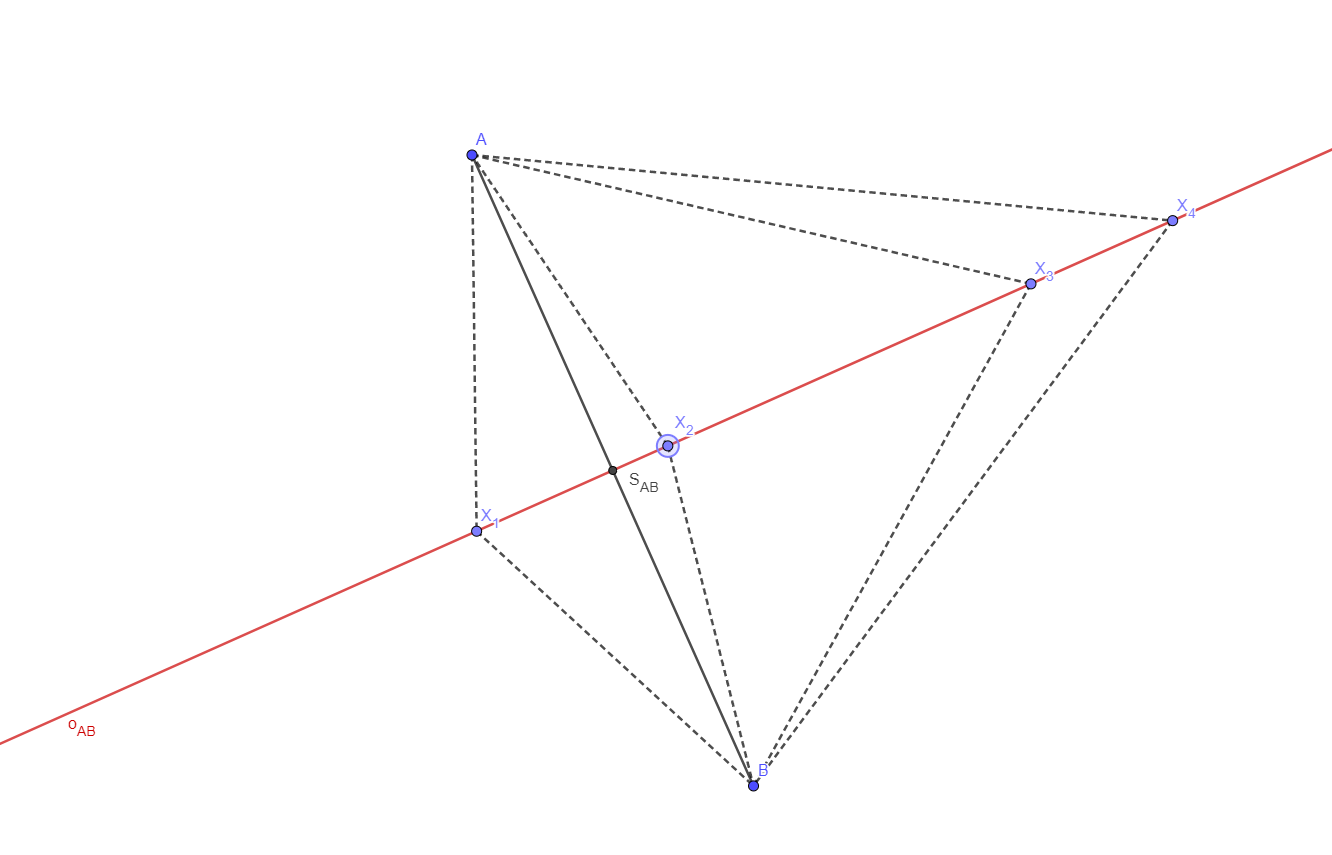
\includegraphics[scale=0.4]{osausecky1}
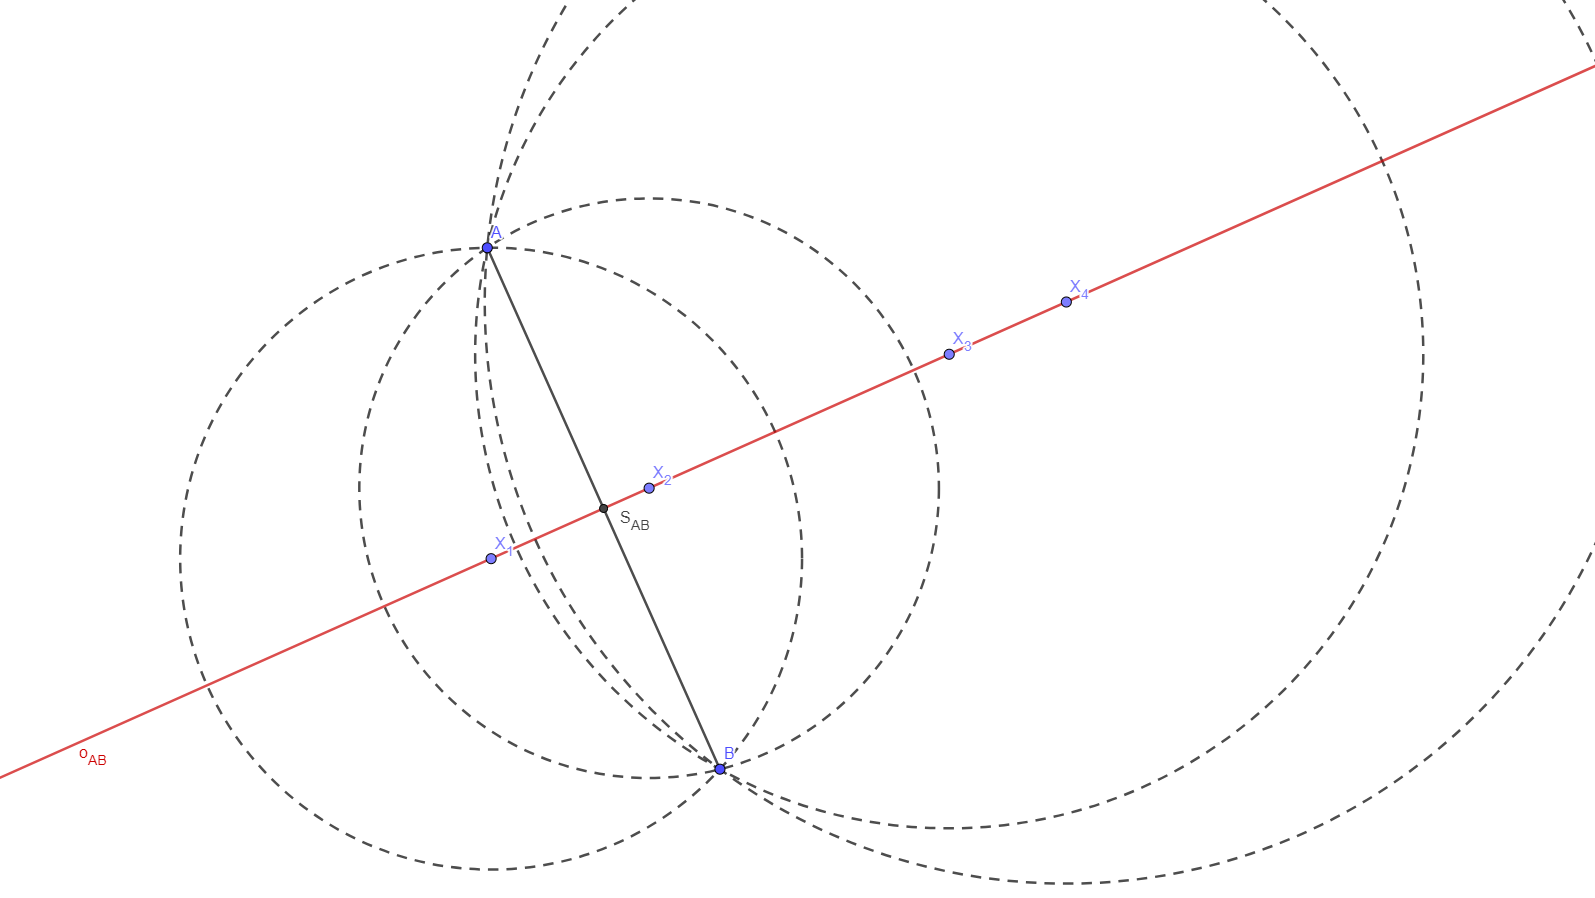
\includegraphics[scale=0.4]{osausecky2}
$o_{AB}=\{X; |AX|=|BX|\}$

\subsection*{Osa rovnoběžek a, b}
Resp. osa rovinného pásu\\
\begin{itemize}
\item je množina všech bodů, které mají od daných dvou rovnoběžek \textit{a,b} stejnou vzdálenost
\item je množina středů všech kružnic, které se dotýkají daných rovnoběžek \textit{a,b}
\end{itemize}

\begin{figure}[H]
\centering
\begin{minipage}{0.5\textwidth}
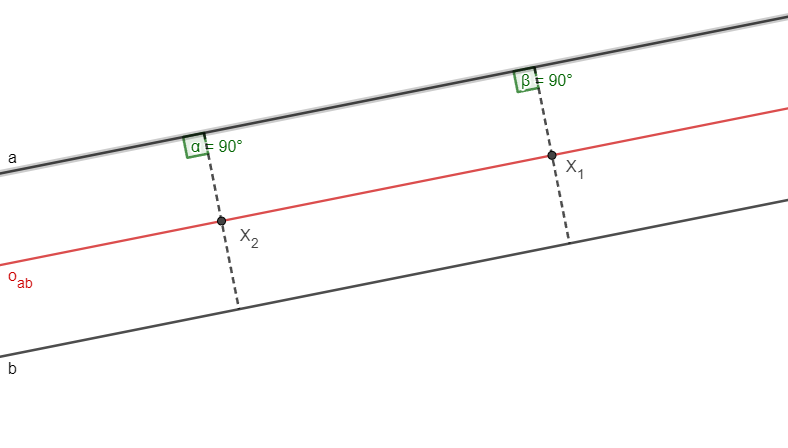
\includegraphics[scale=0.47]{osarovnobezek1}
\end{minipage}%
\vspace{3cm}
\begin{minipage}{0.5\textwidth}
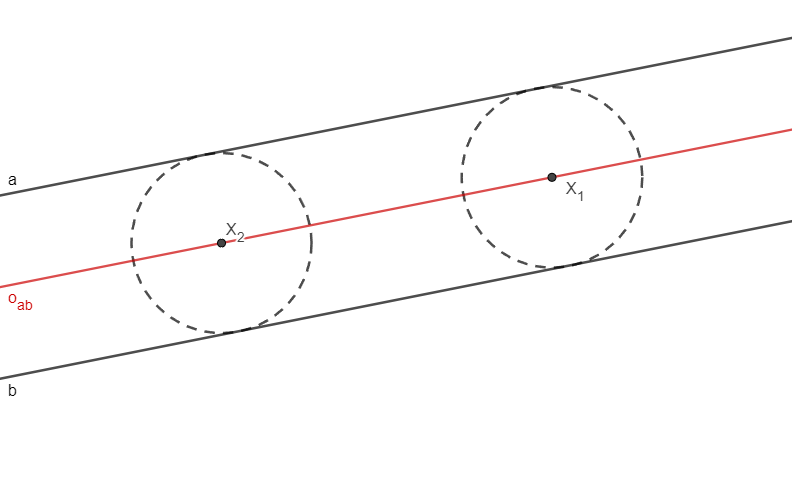
\includegraphics[scale=0.47]{osarovnobezek2}
\end{minipage}
\end{figure}

$o_{ab}=\{X; |Xa|=|Xb|=\frac{1}{2}ab\}$\\

\subsection*{Osy různoběžek}
\begin{itemize}
\item je množina všech bodů, které mají od daných různoběžek \textit{a,b} stejnou vzdálenost
\item (kromě jejich průsečíku) je množina všech středů kružnic, které se dotýkají daných dvou různoběžek \textit{a,b}
\end{itemize}

\begin{figure}[H]
\centering
\begin{minipage}{0.5\textwidth}
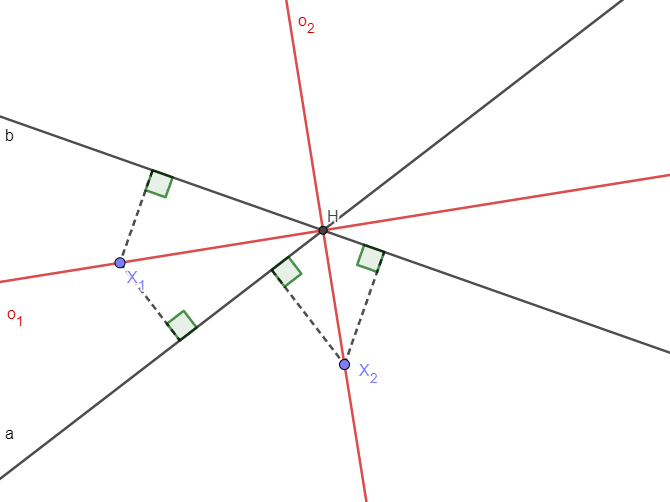
\includegraphics[scale=0.47]{osaruznobezek1}
\end{minipage}%
\vspace{3cm}
\begin{minipage}{0.5\textwidth}
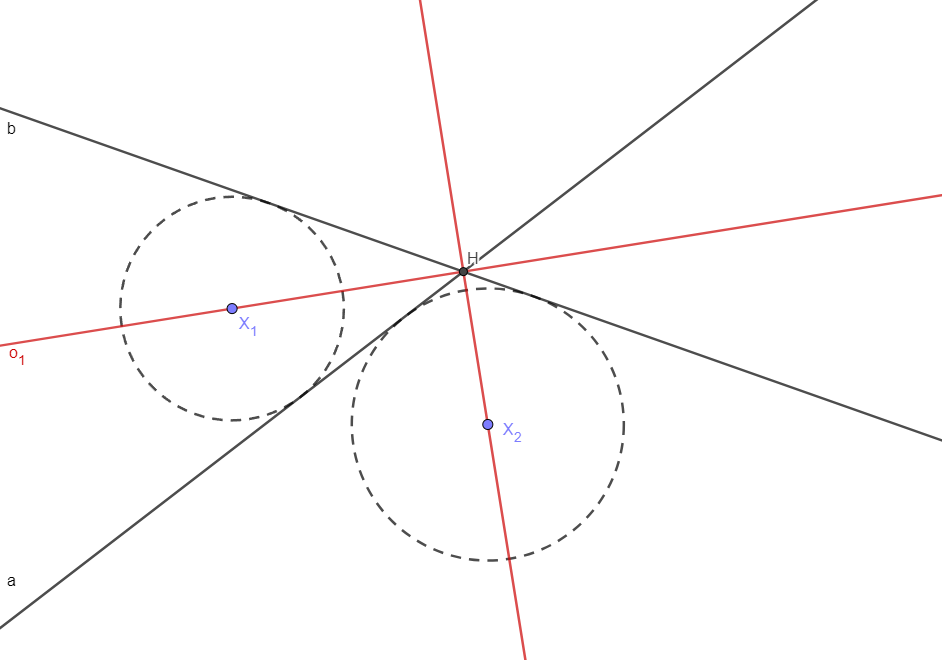
\includegraphics[scale=0.4]{osaruznobezek2}
\end{minipage}
\end{figure}

$o_1 \cup o_2 = \{ X; |Xa|= |Xb|\}$\\
Osy různoběžek jsou na sebe vždy kolmé.

\subsection*{Soustředné kružnice}
Nechť jsou dány dvě soustředné kružnice $k_1(S,r_1), k_2(S, r_2), r_1 > r_2$.\\
\textbf{Kružnice} $k(S,r)$ kde $r=\frac{1}{2}(r_1+r_2)$, je množina všech bodů, které mají od daných kružnic stejnou vzdálenost.\\
\begin{figure}[H]
\centering
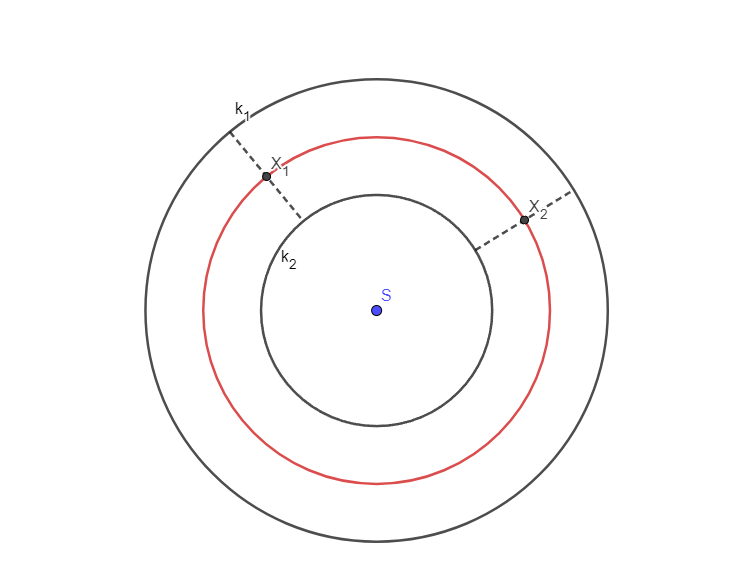
\includegraphics[scale=0.47]{soustredne1}
\end{figure}

\textbf{Dvě kružnice} $k(S, r_1), l(S, r_2)$, kde $r_1=\frac{1}{2}(r_1+r_2), r_2=\frac{1}{2}(r_1-r_2)$ je množina středů kružnic, které se dotýkají daných kružnic. 
\begin{figure}[H]
\centering
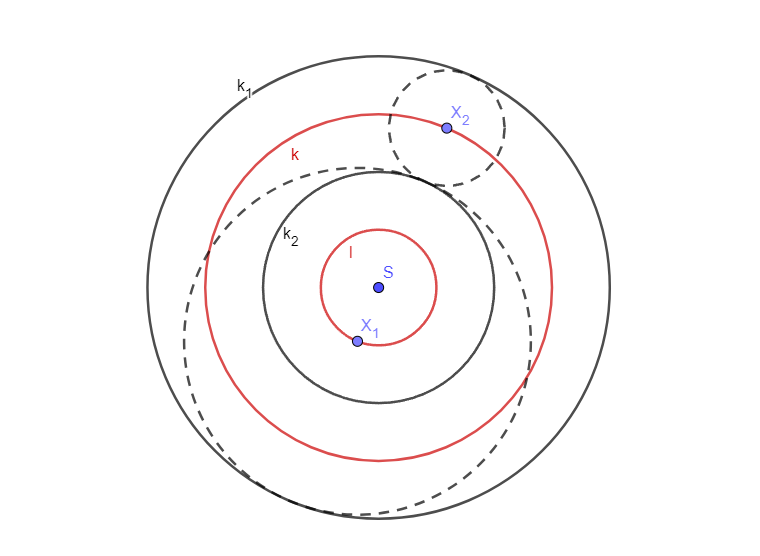
\includegraphics[scale=0.47]{soustredne2}
\end{figure}

\pagebreak

\subsection*{Ekvidistanty kružnice}
Nechť je dána kružnice $k(S,r)$ a kladné reálné číslo \textit{d}.\\
Pro $d < r$ sjednocení kružnic $k_1(S, r+d) \cup k_2(S, r-d)$; pro $d \geq r$ kružnice $k_1(S,r+d)$ je
\begin{itemize}
\item množina všech bodů, které mají od dané kružnice \textit{k} vzdálenost \textit{d}
\item množina středů všech kružnic s poloměrem \textit{d}, které se dotýkají dané kružnice
\end{itemize}
\begin{figure}[H]
\begin{minipage}{0.5\textwidth}
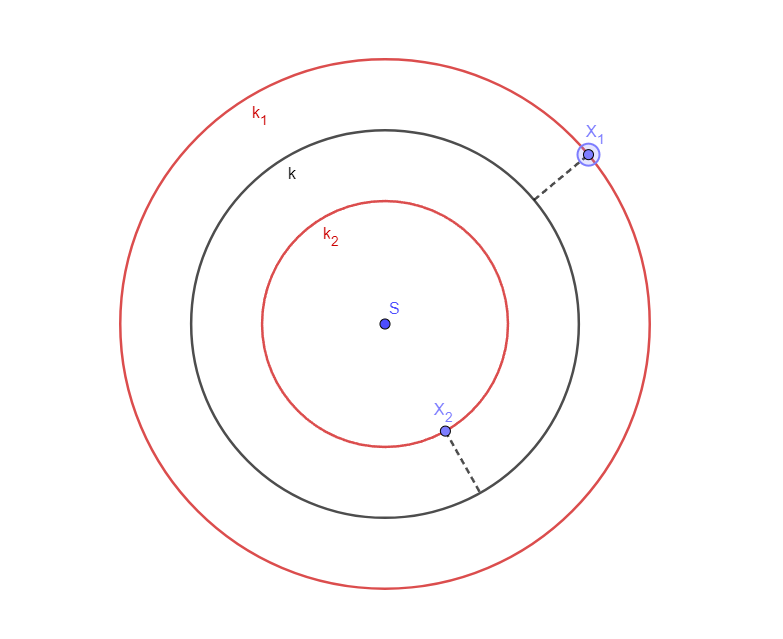
\includegraphics[scale=0.38]{ekvidistantykruznice1}
\end{minipage}%
\begin{minipage}{0.5\textwidth}
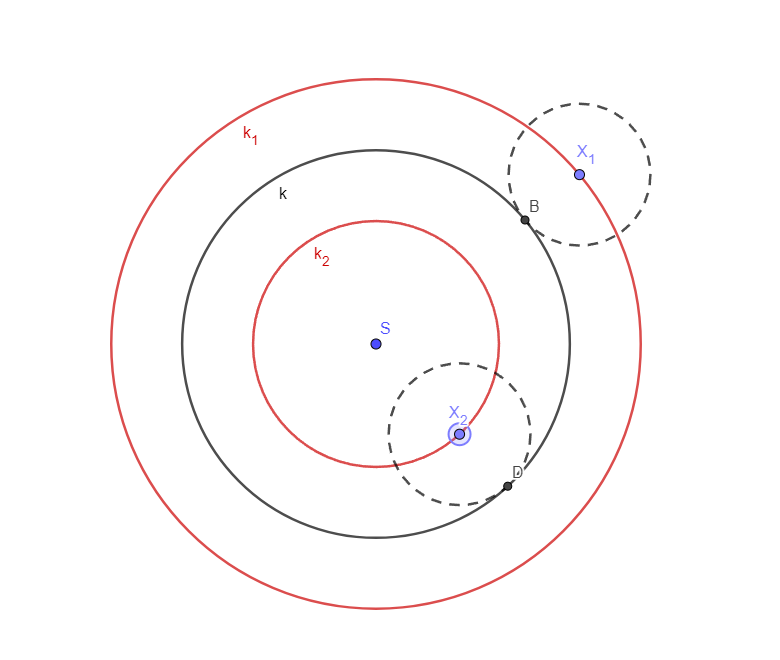
\includegraphics[scale=0.4]{ekvidistantykruznice2}
\end{minipage}
\end{figure}

\pagebreak

\section{Konstrukce trojúhelníků a čtyřúhelníků}
Řešení konstrukční úlohy má tyto fáze:\\
\begin{itemize}
\item \textbf{rozbor úlohy} - předpokládáme že existuje alespoň jeden hledaný trojúhelník, ten načrtneme a vyznačíme hledané prvky; hledáme vztahy a množiny bodů
\item \textbf{zápis konstrukce} - symbolický zápis všech kroků kontrukce (+ pomocný náčrtek)
\item \textbf{konstrukce} - sestrojíme trojúhelník (všechna řešení nebo jen zvolenou polorovinu) podle zápisu
\item \textbf{závěr} - uvedeme počet řešení, popř. zkouška
\end{itemize}

\rule{13.5cm}{0.4pt}

\textbf{\color{green} Sestroj trojúhelník \textit{ABC}, je-li dáno: $a=6cm, b = 5cm, \beta = 50 \degree $.} \color{black}\\
\textbf{Rozbor úlohy:} po sestrojení strany \textit{BC} s délkou 6 cm, musíme najít vrchol \textit{A}, který je od vrcholu \textit{C} vzdálen 5 cm, leží tedy na kružnici $k(C, 5cm)$;
dále víme, že vrchol \textit{A} leží na polopřímce \textit{BX} tak, že velikost úhlu \textit{XBC} je $50 \degree$; vrchol \textit{A} leží v průsečíku množin bodů polopřímky \textit{BX} 
a kružnice \textit{k}. 

\begin{figure}[H]
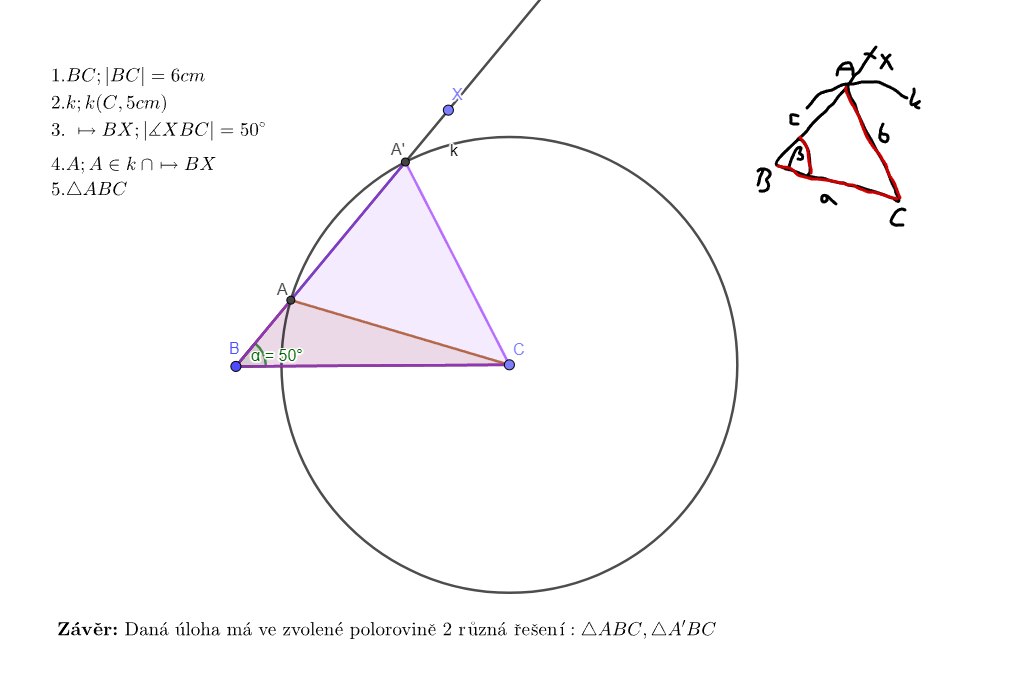
\includegraphics[scale=0.5]{konstrukce1}
\end{figure}
Pokud nejsou zadány údaje konkrétně, ale pouze obecně, konstrukce se neprovádí a místo závěru se provede \textbf{diskuse řešitelnosti}.\\
U $\triangle ABC$ by vypadala: $a > 0, 0 \degree < \beta < 180\degree$; jedno řešení: $\beta < 90\degree \land b = a \sin \beta$ nebo $\beta \geq 90 \degree \land b > a$;
dvě různá řešení: $\beta < 90\degree \land b > a \sin \beta$.

\section{Shodná zobrazení}

Zobrazení \textit{Z} v rovině je předpis, který každému bodu \textit{X} roviny přiřazuje právě jeden bod \textit{X'} roviny. Bod \textit{X} nazýváme \textbf{vzor}, bod \textit{X'} jeho \textbf{obraz}. Zápis: $Z: X \rightarrow X'$.\\
Bod \textit{X}, pro něhož obraz \textit{X'} platí, že $X = X'$, nazýváme \textbf{samodružný}. Zobrazení, ve kterém je každý bod samodružný nazýváme \textbf{identita}.\\

Zobrazení nazýváme \textbf{shodné zobrazení} (nebo též \textbf{shodnost}), právě když obrazem každé úsečky \textit{AB} je úsečka \textit{A'B'} shodná s \textit{AB}.\\
Pokud ověřujeme shodnost dvou útvarů, a pouze průsvitku otáčíme nebo posouváme, mluvíme o \textbf{přímé shodnosti}. Pokud průsvitku převrátíme na druhou stranu, mluvíme o
\textbf{nepřímé shodnosti}.\\
V každém  shodném zobrazení platí:\\
\begin{itemize}
\item obrazem přímky je přímka; obrazem rovnoběžek jsou rovnoběžky
\item obrazem polopřímky je polopřímka; obrazem opačných polopřímek jsou opačné polopřímky
\item obrazem úhlu \textit{AVB} je úhel \textit{A'V'B'}, který je shodný s úhlem \textit{AVB}
\end{itemize}

\subsection*{Osová souměrnost}
\textbf{Osová souměrnost s osou o} (zapisujeme $O(o): X \rightarrow X'$) je shodné zobrazení, které přiřazuje:\\
\begin{itemize}
\item každému bodu $X \notin o$ obraz $X'$ tak, že úsečka $XX'$ je kolmá na osu \textit{o} a střed úsečky $XX'$ leží na ose o
\item každému bodu $X \in o$ obraz $X'$ tak, že $X = X'$
\end{itemize}

\subsection*{Středová souměrnost}
\textbf{Středová souměrnost se středem S} (zapisujeme $S(S): X \rightarrow X'$) je shodné zobrazení. které přiřazuje:\\
\begin{itemize}
\item každému bodu $X \neq S$ obraz $X'$ tak, že bod $S$ je středem úsečky $XX'$
\item bodu $S$ bod $S'=S$
\end{itemize}

\subsection*{Orientovaná úsečka}
\textbf{Orientovaná úsečka }$\overrightarrow{\rm AB}$ je úsečka, u které rozlišujeme počáteční bod \textit{A} a koncový bod \textit{B} (vpodstatě vektor).\\
\textbf{Velikost} orientované úsečky je definována jako $|AB|$.\\
\textbf{Nulová orientovaná úsečka} má nulovou velikost a její počáteční i koncový bod splývají.\\
Jsou-li dvě orientované úsečky rovnoběžné, říkáme, že mají \textbf{stejný směr}. Navíc říkáme, že jsou:\\
\begin{figure}[H]
\centering
\begin{minipage}{0.45\textwidth}
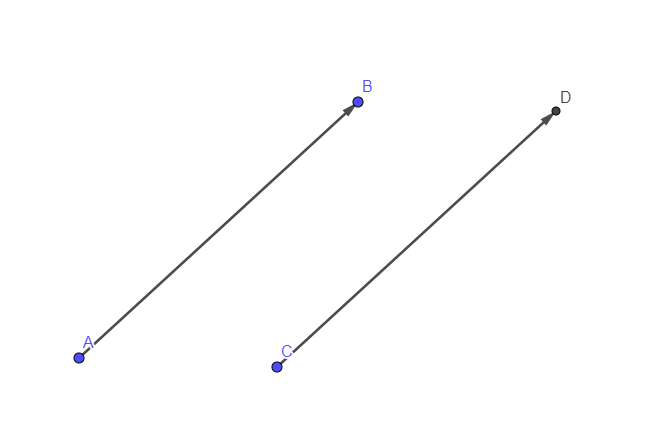
\includegraphics[scale=0.4]{orient1}
\subcaption{souhlasně orientované}
\end{minipage}
\begin{minipage}{0.45\textwidth}
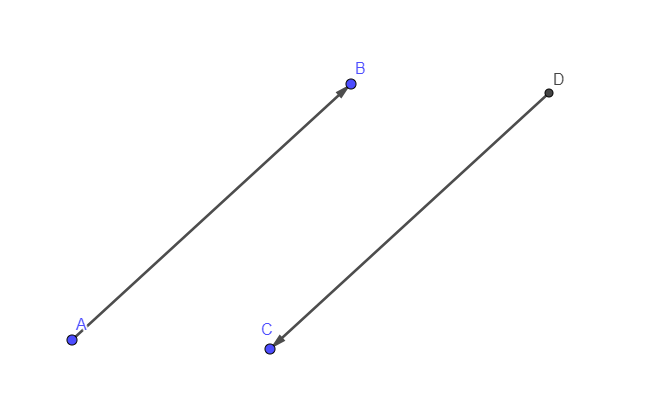
\includegraphics[scale=0.4]{orient2}
\subcaption{nesouhlasně orientované}
\end{minipage}
\end{figure} 

\subsection*{Translace}
\textbf{Posunutí} (zapisujeme $T(\overrightarrow{\rm AB}): X \rightarrow X'$) je shodné zobrazení, které přiřazuje každému bodu $X$ obraz $X'$ tak, že úsečky $\overrightarrow{\rm AB}$ a 
$\overrightarrow{\rm XX'}$ mají stejný směr, orientaci a velikost.\\
\begin{figure}[H]
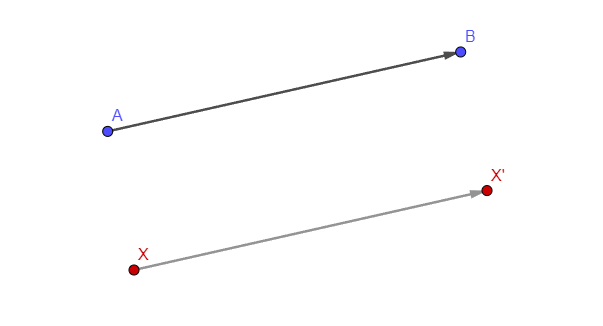
\includegraphics[scale=0.8]{translace}
\end{figure}

\section{Podobná zobrazení}
tady cekam na floru, protoze asi nemam ty archy? jako vim co to je, takovy to homotetie, rotace a tak ale idk zapis k tomu zejo
\section{Pythagorova a Eukleidovy věty}

\subsection*{Pythagorova věta}
\textit{Obsah čtverce sestrojeného nad přeponou pravoúhlého trojúhelníku je roven součtu obsahu čtverců sestrojených nad oběma odvěsnami.}\\
Symbolicky zapisujeme: $c^2=a^2+b^2$, kde \textit{c} je přepona.\\
Znění věty lze rozšířit i na např. půlkruhy.

\begin{figure}[H]
\centering
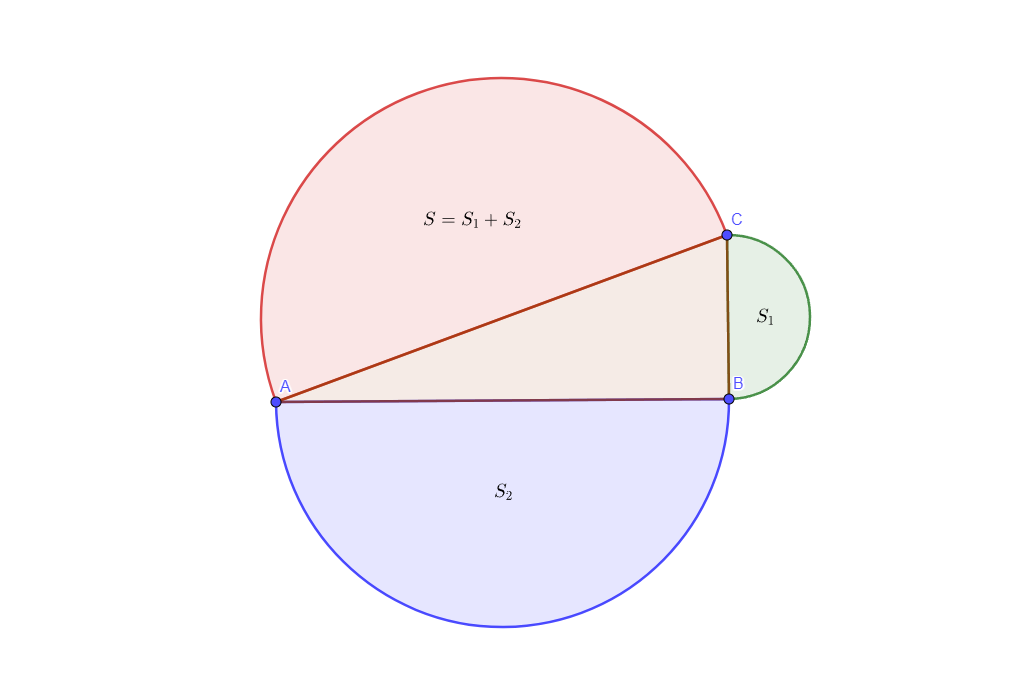
\includegraphics[scale=0.3]{pv1}
\end{figure}

\subsection*{Eukleidovy věty}
Výška v pravoúhlém trojuhelníku je vzdálenost vrcholu při pravém úhlu od přímky, na níž leží přepona. Pata \textit{P} výšky rozdělí přeponu na dva úseky $c_a$ a $c_b$.
\subsubsection*{Eukleidova věta o výšce}
\textit{Obsah čtverce sestrojeného nad výškou pravoúhlého trojúhelníku je roven obsahu obdélníku, jehož strany tvoří oba úseky přepony.}\\
\begin{center}
$v^2=c_a \cdot c_b$
\end{center}
\begin{figure}[H]
\centering
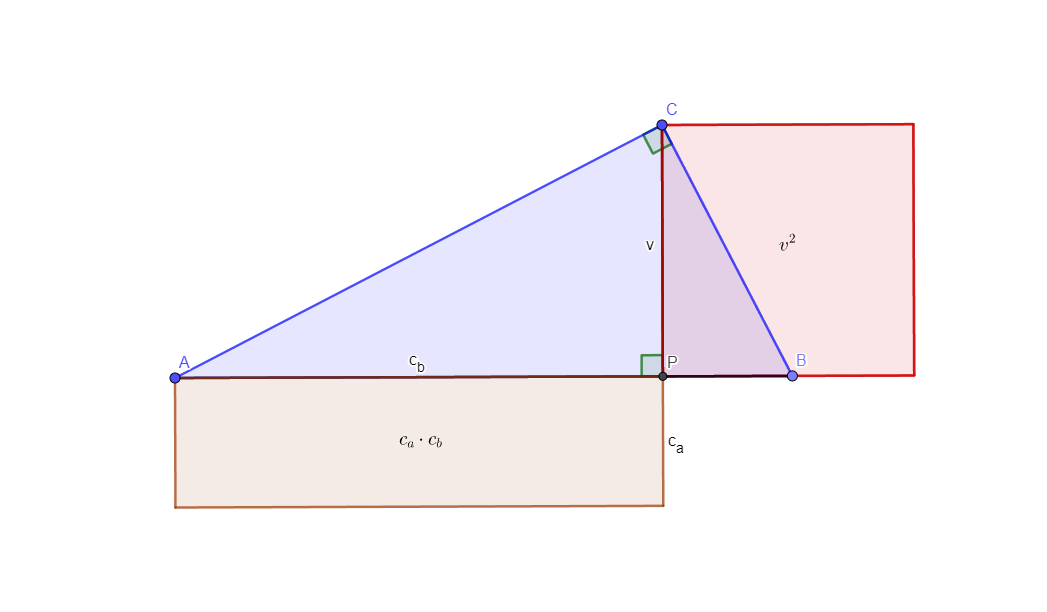
\includegraphics[scale=0.3]{evv}
\end{figure}
\subsubsection*{Eukleidova věta o odvěsně}
\textit{Obsah čtverce sestrojeného nad odvěsnou pravoúhlého trojúhelníku je roven obsahu obdélníku, jehož strany tvoří přepona a přilehlý úsek.}\\
\begin{center}
$a^2 = c \cdot c_a \lor b^2 = c \cdot c_b$
\end{center}
\begin{figure}[H]
\centering
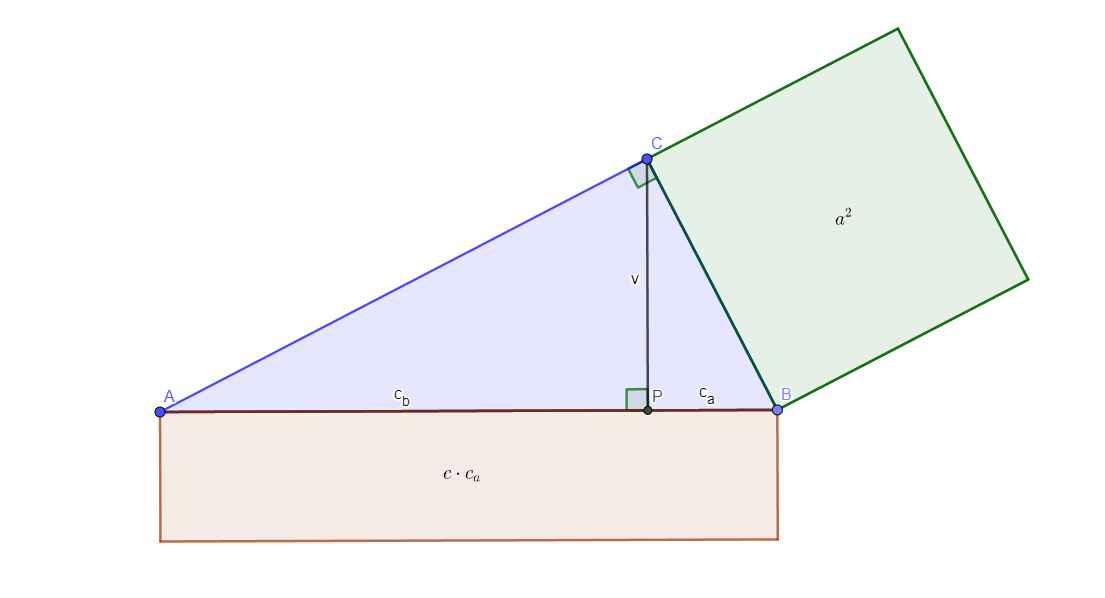
\includegraphics[scale=0.3]{evo}
\end{figure}

\subsection*{Převod trojúhelníku na obdélník}
Máme-li bez výpočtu sestrojit obdélník, který má stejný obsah jako daný trojúhelník, využijeme obsah trojúhelníku: $S = \frac{a\cdot v_a}{2}$ a upravíme jej na tvar 
$S = a \cdot \frac{v_a}{2}$. Sestrojit úsečku $b = \frac{v_a}{2}$ lze pomocí kružítka a pravítka. Máme vzorec $S = a \cdot b$, což je obsah obdélníku se stranami $a,b=\frac{1}{2}v_a$.\\
\begin{figure}[H]
\centering
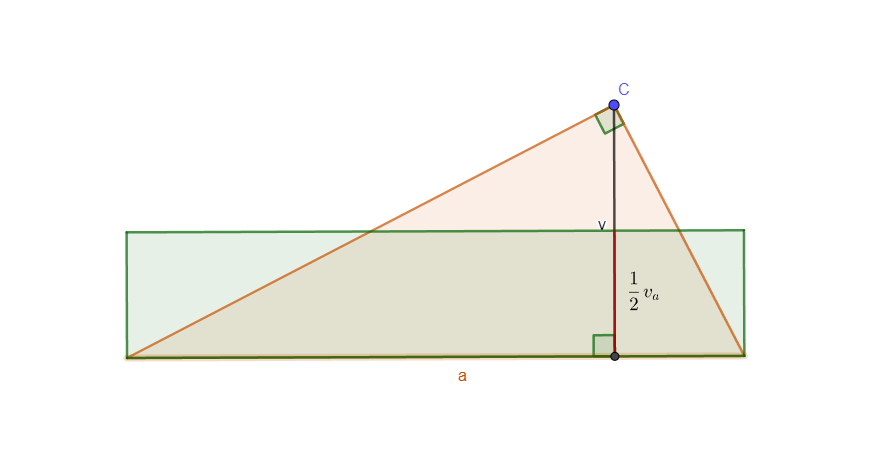
\includegraphics[scale=0.6]{prevodtnaob}
\end{figure}

\pagebreak

\subsection*{Převod obdélníku na čtverec}
Jsou dva způsoby převodu:\\
\subsubsection*{První s využitím EVV}
Sestrojíme úsečku \textit{AB} délky $a+b$ a nad ní Thaletovu kružnici. Bodem \textit{P} (dělí \textit{AB} na dva úseky) sestrojíme kolmici na \textit{AB}. Průsečík s kružnicí označíme 
\textit{C}. $\triangle ABC$ je pravoúhlý, \textit{AB} je přepona a úsečka \textit{CP} výška. Z EVV plyne: $|AP|\cdot |BP|=|CP|^2 \imply a \cdot = v^2$ a výška má velikost $v=\sqrt{ab}$
\begin{figure}[H]
\centering
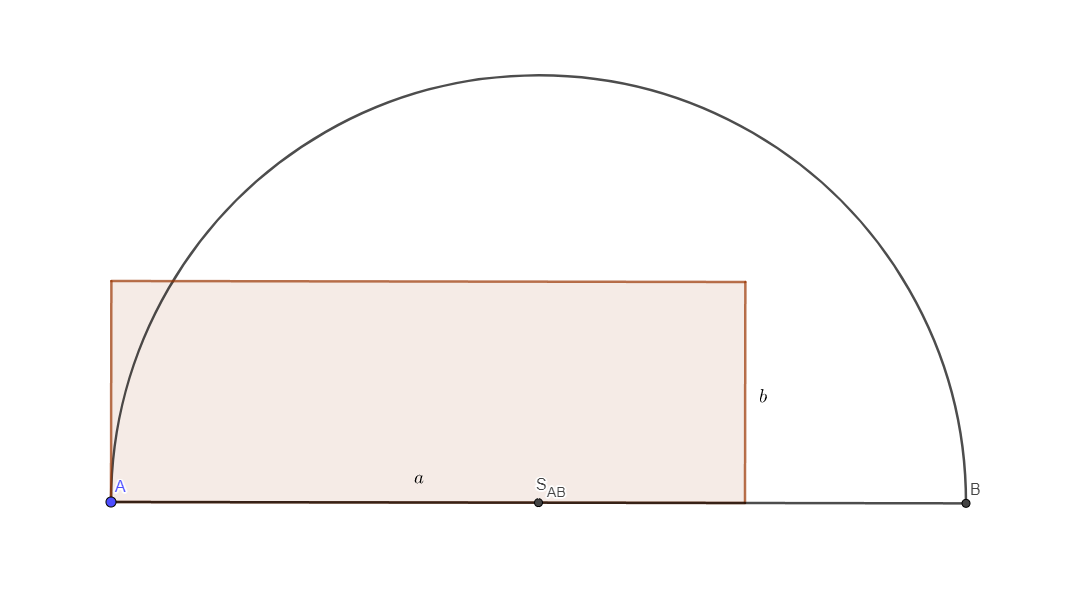
\includegraphics[scale=0.3]{ponc1}
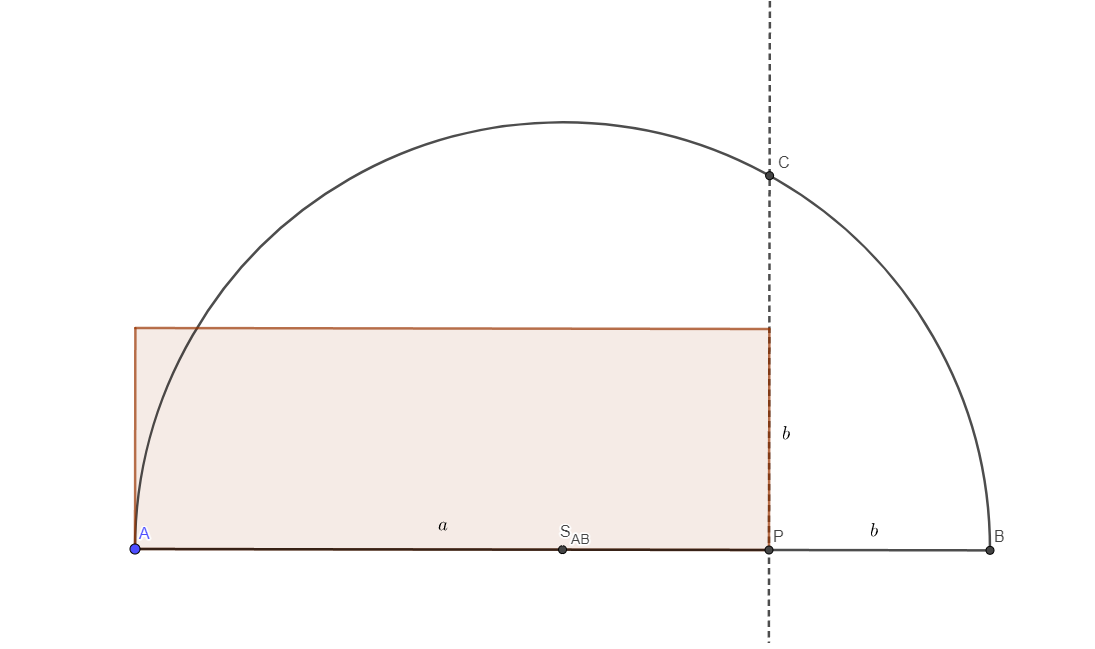
\includegraphics[scale=0.3]{ponc2}
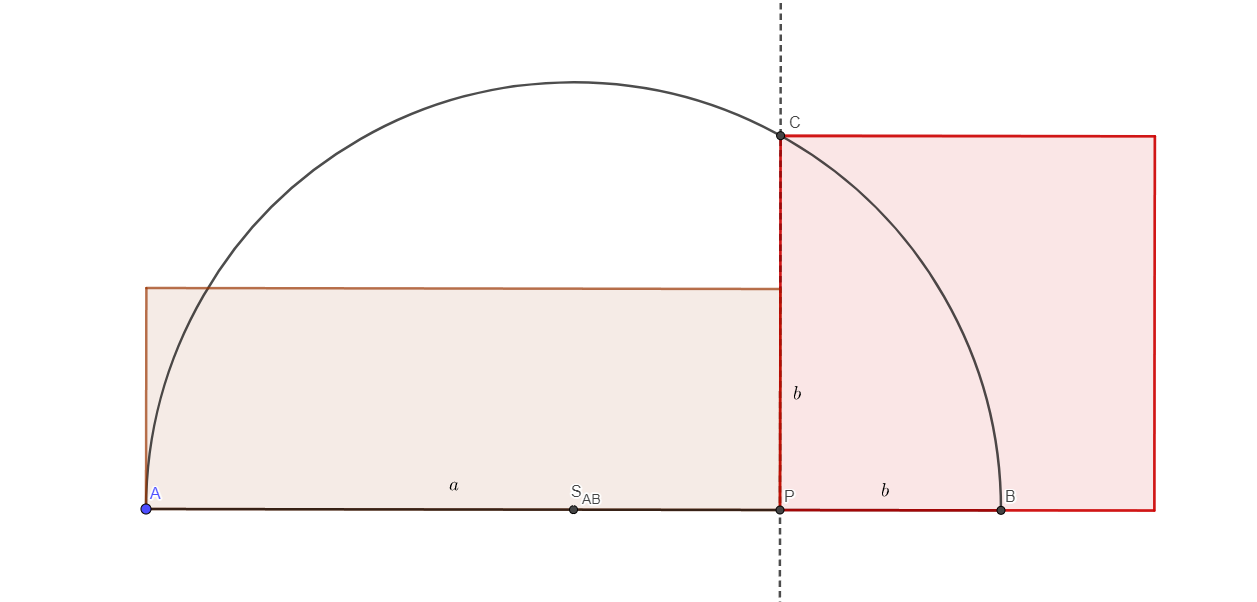
\includegraphics[scale=0.3]{ponc3}
\end{figure} 
\subsubsection*{Druhý s využitím EVO}
Delší stranu obdélníku označíme \textit{AB} a zvolíme na ní pod \textit{P} tak, aby $|PB| = b$. Nad \textit{AB} sestrojíme Thaletovu kružnici a bodem \textit{P} kolmici k \textit{AB}.
Průsečík komice a kružnice označíme \textit{C}. $\triangle ABC$ je pravoúhlý s přeponou \textit{AB}, odvěsnou \textit{BC} a přilehlým úsekem \textit{PB}. 
Z EVO plyne: $|AP|\cdot |BP|= |BC|^2 \imply a \cdot b = x^2$, úsečka $x=\sqrt{ab}$. 

\begin{figure}[H]
\centering
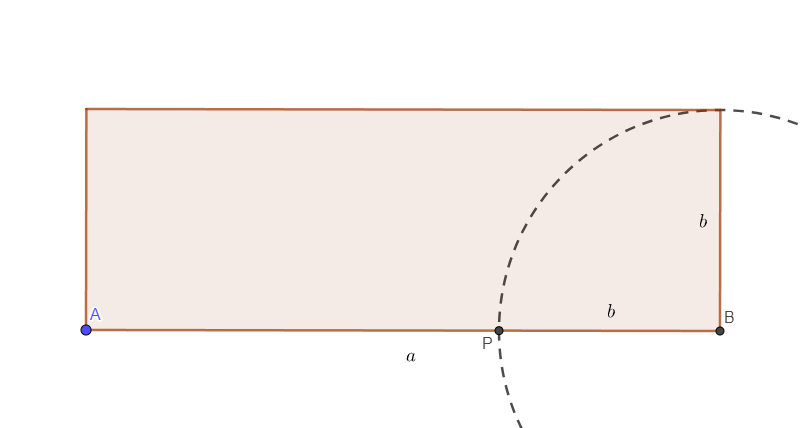
\includegraphics[scale=0.35]{ponc4}
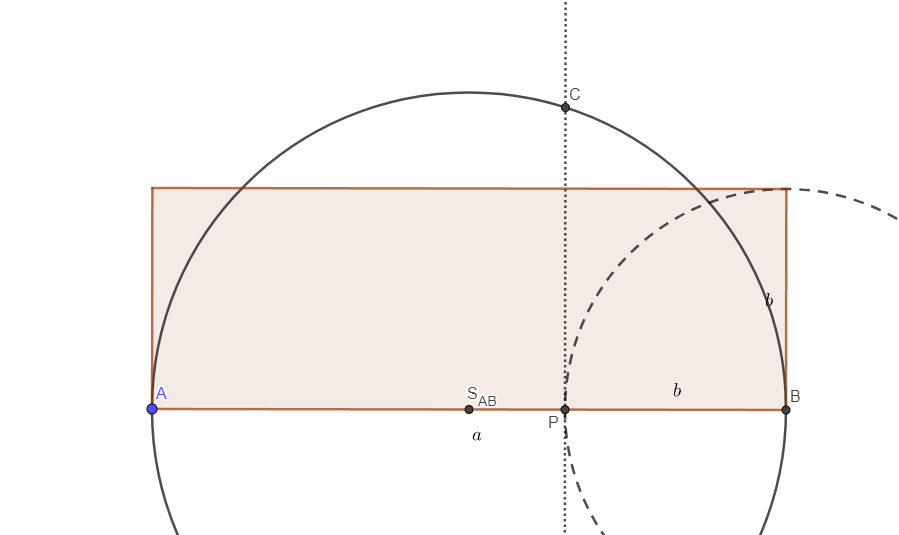
\includegraphics[scale=0.35]{ponc5}
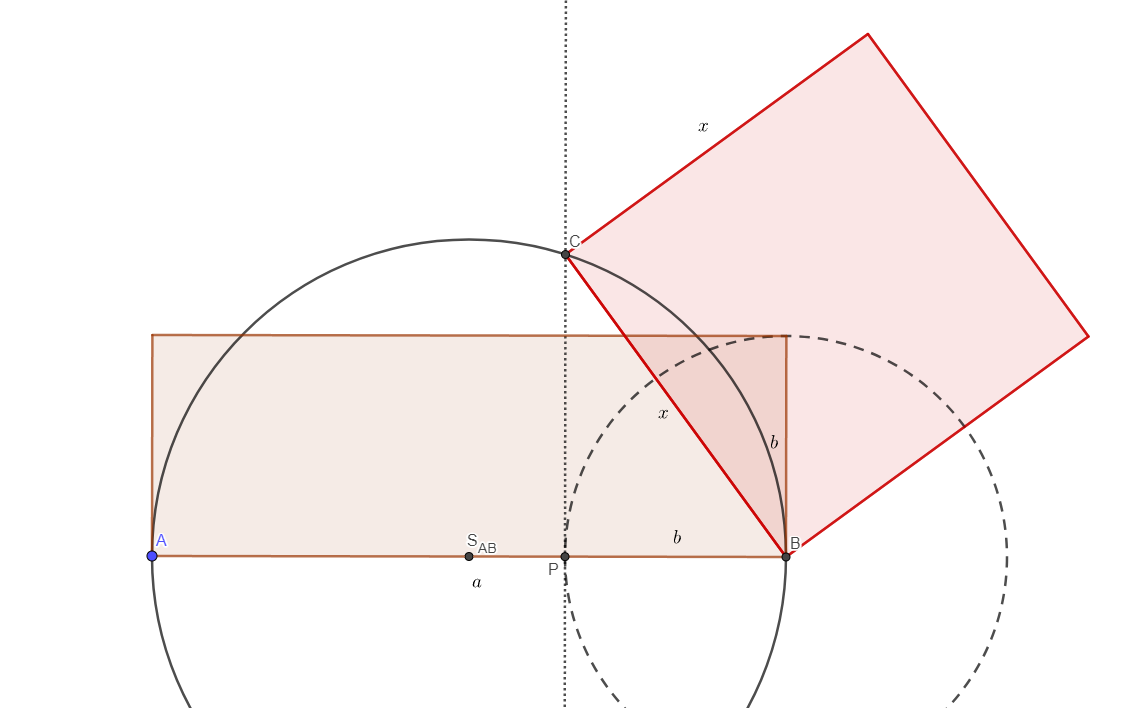
\includegraphics[scale=0.35]{ponc6}
\end{figure} 

\section{Trigonometrie obecného trojúhelníku}
Nechť je dán libovolný trojúhleník \textit{ABC} se stranami \textit{a,b,c} a vnitřními úhly $\alpha,\beta,\gamma$. Pak platí:
\subsection*{Sinová věta}
\begin{center}
$\frac{a}{b}=\frac{\sin \alpha}{\sin \beta} \lor \frac{a}{c}=\frac{\sin \alpha}{\sin \gamma} \lor \frac{b}{c}=\frac{\sin \beta}{\sin \gamma}$\\
souhrnně: $a:b:c = \sin \alpha : \sin \beta : \sin \gamma$
\end{center}

\subsection*{Kosinová věta}
$c^2=a^2+b^2-2ab\cos \gamma$, resp.\\
$b^2=a^2+c^2-2ac\cos \beta$, resp.\\
$a^2=b^2+c^2-2bc\cos \alpha$

\subsection*{Obsah a poloměry}
\begin{itemize}
\item \textbf{obsah} $\triangle ABC$ je roven: $S = \frac{1}{2}ab\sin \gamma$, resp. $S = \frac{1}{2}ac\sin \beta$
\item \textbf{poloměr kružnice vepsané} je roven: $\rho = \frac{S}{s}$, kde $s=\frac{1}{2}(a+b+c)$
\item \textbf{poloměr kružnice opsané} je roven: $r = \frac{a}{2\sin \alpha}=\frac{b}{2\sin \beta}=\frac{c}{2\sin \gamma}$
\end{itemize}

\subsection*{Úhly při slovních úlohách}
\begin{figure}[H]
\centering
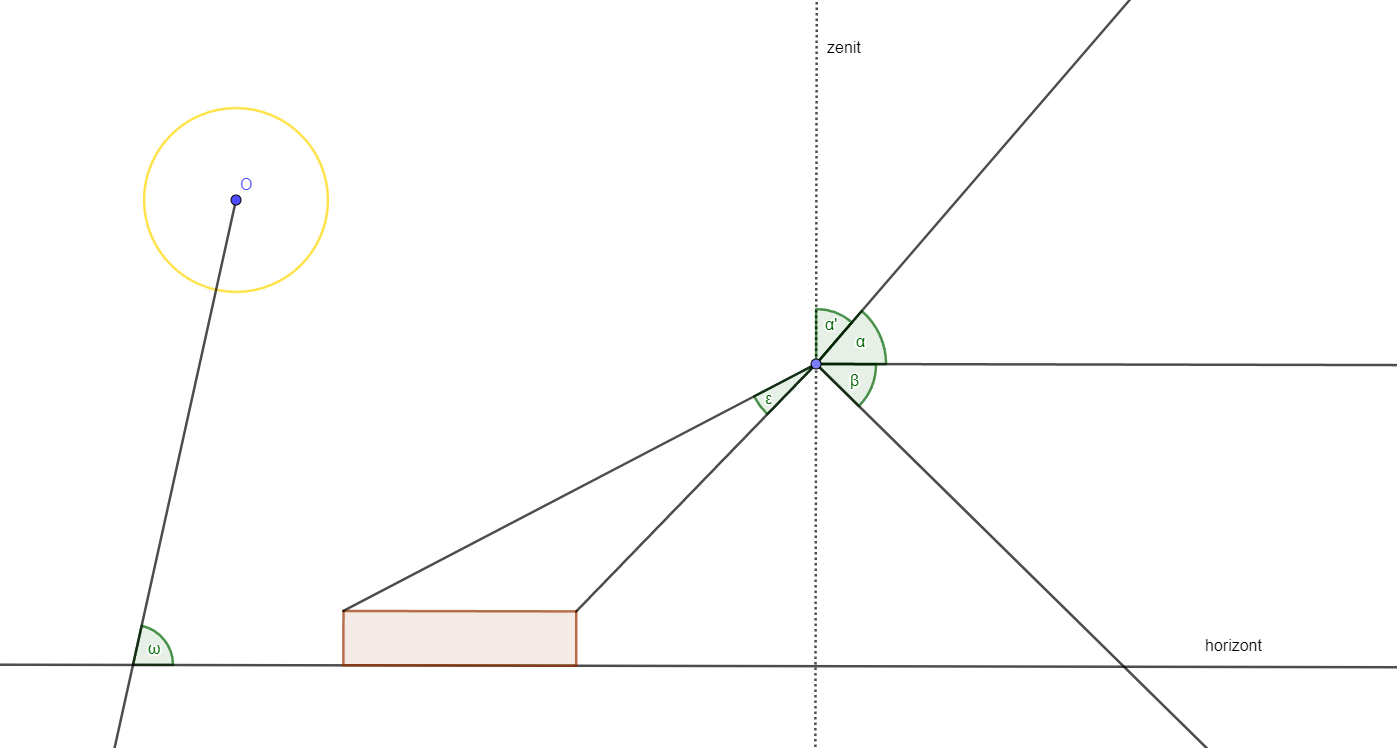
\includegraphics[scale=0.3]{vyskovyuhel}
\vspace{2cm}
\begin{itemize}
\item $\omega$ ... výška nad obzorem
\item $\alpha$ ... výškový úhel
\item $\alpha'$ ... zenitový úhel
\item $\beta$ ... hloubkový úhel
\item $\epsilon$ ... zorný úhel
\end{itemize}
\end{figure} 

\section{Stereometrie – polohové vlastnosti}
\section{Stereometrie – metrické vlastnosti}
\section{Stereometrie – objem a povrch těles}
\section{Analytická geometrie – body a vektory}
\section{Analytická geometrie – přímka a polorovina v E2}
\section{Analytická geometrie – přímka a rovina v E3}
\section{Analytická geometrie – kuželosečky}
\section{Kombinatorika}
\section{Pravděpodobnost}
\section{Statistika}
\section{Posloupnosti}
\section{Limita posloupnosti a nekonečná geometrická řada}
\section{Limita a derivace funkce}



\end{document}